%  LaTeX support: latex@mdpi.com 
%  For support, please attach all files needed for compiling as well as the log file, and specify your operating system, LaTeX version, and LaTeX editor.

%=================================================================
\documentclass[journal,article,submit,pdftex,moreauthors]{Definitions/mdpi} 
%\documentclass[preprints,article,submit,pdftex,moreauthors]{Definitions/mdpi} 
% For posting an early version of this manuscript as a preprint, you may use "preprints" as the journal. Changing "submit" to "accept" before posting will remove line numbers.

% Below journals will use APA reference format:
% admsci, behavsci, businesses, econometrics, economies, education, ejihpe, famsci, games, humans, ijcs, ijfs, journalmedia, jrfm, languages, psycholint, publications, tourismhosp, youth

% Below journals will use Chicago reference format:
% arts, genealogy, histories, humanities, jintelligence, laws, literature, religions, risks, socsci

%--------------------
% Class Options:
%--------------------
%----------
% journal
%----------
% Choose between the following MDPI journals:
% accountaudit, acoustics, actuators, addictions, adhesives, admsci, adolescents, aerobiology, aerospace, agriculture, agriengineering, agrochemicals, agronomy, ai, air, algorithms, allergies, alloys, amh, analytica, analytics, anatomia, anesthres, animals, antibiotics, antibodies, antioxidants, applbiosci, appliedchem, appliedmath, appliedphys, applmech, applmicrobiol, applnano, applsci, aquacj, architecture, arm, arthropoda, arts, asc, asi, astronomy, atmosphere, atoms, audiolres, automation, axioms, bacteria, batteries, bdcc, behavsci, beverages, biochem, bioengineering, biologics, biology, biomass, biomechanics, biomed, biomedicines, biomedinformatics, biomimetics, biomolecules, biophysica, biosensors, biosphere, biotech, birds, blockchains, bloods, blsf, brainsci, breath, buildings, businesses, cancers, carbon, cardiogenetics, catalysts, cells, ceramics, challenges, chemengineering, chemistry, chemosensors, chemproc, children, chips, cimb, civileng, cleantechnol, climate, clinbioenerg, clinpract, clockssleep, cmd, cmtr, coasts, coatings, colloids, colorants, commodities, complications, compounds, computation, computers, condensedmatter, conservation, constrmater, cosmetics, covid, crops, cryo, cryptography, crystals, csmf, ctn, curroncol, cyber, dairy, data, ddc, dentistry, dermato, dermatopathology, designs, devices, diabetology, diagnostics, dietetics, digital, disabilities, diseases, diversity, dna, drones, dynamics, earth, ebj, ecm, ecologies, econometrics, economies, education, eesp, ejihpe, electricity, electrochem, electronicmat, electronics, encyclopedia, endocrines, energies, eng, engproc, ent, entomology, entropy, environments, epidemiologia, epigenomes, esa, est, famsci, fermentation, fibers, fintech, fire, fishes, fluids, foods, forecasting, forensicsci, forests, fossstud, foundations, fractalfract, fuels, future, futureinternet, futureparasites, futurepharmacol, futurephys, futuretransp, galaxies, games, gases, gastroent, gastrointestdisord, gastronomy, gels, genealogy, genes, geographies, geohazards, geomatics, geometry, geosciences, geotechnics, geriatrics, glacies, grasses, greenhealth, gucdd, hardware, hazardousmatters, healthcare, hearts, hemato, hematolrep, heritage, higheredu, highthroughput, histories, horticulturae, hospitals, humanities, humans, hydrobiology, hydrogen, hydrology, hygiene, idr, iic, ijerph, ijfs, ijgi, ijmd, ijms, ijns, ijpb, ijt, ijtm, ijtpp, ime, immuno, informatics, information, infrastructures, inorganics, insects, instruments, inventions, iot, j, jal, jcdd, jcm, jcp, jcs, jcto, jdad, jdb, jeta, jfb, jfmk, jimaging, jintelligence, jlpea, jmahp, jmmp, jmms, jmp, jmse, jne, jnt, jof, joitmc, joma, jop, jor, journalmedia, jox, jpbi, jpm, jrfm, jsan, jtaer, jvd, jzbg, kidney, kidneydial, kinasesphosphatases, knowledge, labmed, laboratories, land, languages, laws, life, lights, limnolrev, lipidology, liquids, literature, livers, logics, logistics, lubricants, lymphatics, machines, macromol, magnetism, magnetochemistry, make, marinedrugs, materials, materproc, mathematics, mca, measurements, medicina, medicines, medsci, membranes, merits, metabolites, metals, meteorology, methane, metrics, metrology, micro, microarrays, microbiolres, microelectronics, micromachines, microorganisms, microplastics, microwave, minerals, mining, mmphys, modelling, molbank, molecules, mps, msf, mti, multimedia, muscles, nanoenergyadv, nanomanufacturing, nanomaterials, ncrna, ndt, network, neuroglia, neurolint, neurosci, nitrogen, notspecified, nursrep, nutraceuticals, nutrients, obesities, oceans, ohbm, onco, oncopathology, optics, oral, organics, organoids, osteology, oxygen, parasites, parasitologia, particles, pathogens, pathophysiology, pediatrrep, pets, pharmaceuticals, pharmaceutics, pharmacoepidemiology, pharmacy, philosophies, photochem, photonics, phycology, physchem, physics, physiologia, plants, plasma, platforms, pollutants, polymers, polysaccharides, populations, poultry, powders, preprints, proceedings, processes, prosthesis, proteomes, psf, psych, psychiatryint, psychoactives, psycholint, publications, purification, quantumrep, quaternary, qubs, radiation, reactions, realestate, receptors, recycling, regeneration, religions, remotesensing, reports, reprodmed, resources, rheumato, risks, robotics, rsee, ruminants, safety, sci, scipharm, sclerosis, seeds, sensors, separations, sexes, signals, sinusitis, siuj, skins, smartcities, sna, societies, socsci, software, soilsystems, solar, solids, spectroscj, sports, standards, stats, std, stresses, surfaces, surgeries, suschem, sustainability, symmetry, synbio, systems, tae, targets, taxonomy, technologies, telecom, test, textiles, thalassrep, therapeutics, thermo, timespace, tomography, tourismhosp, toxics, toxins, transplantology, transportation, traumacare, traumas, tropicalmed, universe, urbansci, uro, vaccines, vehicles, venereology, vetsci, vibration, virtualworlds, viruses, vision, waste, water, wem, wevj, wild, wind, women, world, youth, zoonoticdis

%---------
% article
%---------
% The default type of manuscript is "article", but can be replaced by: 
% abstract, addendum, article, benchmark, book, bookreview, briefcommunication, briefreport, casereport, changes, clinicopathologicalchallenge, comment, commentary, communication, conceptpaper, conferenceproceedings, correction, conferencereport, creative, datadescriptor, discussion, entry, expressionofconcern, extendedabstract, editorial, essay, erratum, fieldguide, hypothesis, interestingimages, letter, meetingreport, monograph, newbookreceived, obituary, opinion, proceedingpaper, projectreport, reply, retraction, review, perspective, protocol, shortnote, studyprotocol, supfile, systematicreview, technicalnote, viewpoint, guidelines, registeredreport, tutorial,  giantsinurology, urologyaroundtheworld
% supfile = supplementary materials

%----------
% submit
%----------
% The class option "submit" will be changed to "accept" by the Editorial Office when the paper is accepted. This will only make changes to the frontpage (e.g., the logo of the journal will get visible), the headings, and the copyright information. Also, line numbering will be removed. Journal info and pagination for accepted papers will also be assigned by the Editorial Office.

%------------------
% moreauthors
%------------------
% If there is only one author the class option oneauthor should be used. Otherwise use the class option moreauthors.

%---------
% pdftex
%---------
% The option pdftex is for use with pdfLaTeX. Remove "pdftex" for (1) compiling with LaTeX & dvi2pdf (if eps figures are used) or for (2) compiling with XeLaTeX.

%=================================================================
% MDPI internal commands - do not modify
\firstpage{1} 
\makeatletter 
\setcounter{page}{\@firstpage} 
\makeatother
\pubvolume{1}
\issuenum{1}
\articlenumber{0}
\pubyear{2025}
\copyrightyear{2025}
%\externaleditor{Firstname Lastname} % More than 1 editor, please add `` and '' before the last editor name
\datereceived{ } 
\daterevised{ } % Comment out if no revised date
\dateaccepted{ } 
\datepublished{ } 
%\datecorrected{} % For corrected papers: "Corrected: XXX" date in the original paper.
%\dateretracted{} % For retracted papers: "Retracted: XXX" date in the original paper.
\hreflink{https://doi.org/} % If needed use \linebreak
%\doinum{}
%\pdfoutput=1 % Uncommented for upload to arXiv.org
%\CorrStatement{yes}  % For updates
%\longauthorlist{yes} % For many authors that exceed the left citation part

%=================================================================
% Add packages and commands here. The following packages are loaded in our class file: fontenc, inputenc, calc, indentfirst, fancyhdr, graphicx, epstopdf, lastpage, ifthen, float, amsmath, amssymb, lineno, setspace, enumitem, mathpazo, booktabs, titlesec, etoolbox, tabto, xcolor, colortbl, soul, multirow, microtype, tikz, totcount, changepage, attrib, upgreek, array, tabularx, pbox, ragged2e, tocloft, marginnote, marginfix, enotez, amsthm, natbib, hyperref, cleveref, scrextend, url, geometry, newfloat, caption, draftwatermark, seqsplit
% cleveref: load \crefname definitions after \begin{document}

%=================================================================
% Please use the following mathematics environments: Theorem, Lemma, Corollary, Proposition, Characterization, Property, Problem, Example, ExamplesandDefinitions, Hypothesis, Remark, Definition, Notation, Assumption
%% For proofs, please use the proof environment (the amsthm package is loaded by the MDPI class).

%=================================================================
% Full title of the paper (Capitalized)
\Title{Real-Time Adaptive TECS Gain Tuning Using Neural Networks for Tiltrotor eVTOL}

% MDPI internal command: Title for citation in the left column
\TitleCitation{Title}

% Author Orchid ID: enter ID or remove command
\newcommand{\orcidauthorA}{0000-0000-0000-000X} % Add \orcidA{} behind the author's name
%\newcommand{\orcidauthorB}{0000-0000-0000-000X} % Add \orcidB{} behind the author's name

% Authors, for the paper (add full first names)
\Author{Choonghyun Lee $^{1,\dagger,\ddagger}$\orcidA{},Ngoc-Phi Nguyen
$^{1,\ddagger}$, Sangjun Bae $^{2,\ddagger}$ and Sungkyung Hong $^{3,}$*}

%\longauthorlist{yes}

% MDPI internal command: Authors, for metadata in PDF
\AuthorNames{Firstname Lastname, Firstname Lastname and Firstname Lastname}

% MDPI internal command: Authors, for citation in the left column, only choose below one of them according to the journal style
% If this is a Chicago style journal 
% (arts, genealogy, histories, humanities, jintelligence, laws, literature, religions, risks, socsci): 
% Lastname, Firstname, Firstname Lastname, and Firstname Lastname.

% If this is a APA style journal 
% (admsci, behavsci, businesses, econometrics, economies, education, ejihpe, games, humans, ijfs, journalmedia, jrfm, languages, psycholint, publications, tourismhosp, youth): 
% Lastname, F., Lastname, F., \& Lastname, F.

% If this is a ACS style journal (Except for the above Chicago and APA journals, all others are in the ACS format): 
% Lastname, F.; Lastname, F.; Lastname, F.
\isAPAStyle{%
       \AuthorCitation{Lastname, F., Lastname, F., \& Lastname, F.}
         }{%
        \isChicagoStyle{%
        \AuthorCitation{Lastname, Firstname, Firstname Lastname, and Firstname Lastname.}
        }{
        \AuthorCitation{Lastname, F.; Lastname, F.; Lastname, F.}
        }
}

% Affiliations / Addresses (Add [1] after \address if there is only one affiliation.)
\address{%
$^{1}$ \quad Department of Convergence Engineering for Intelligent Drone, Sejong University; chungh6577@sju.ac.kr\\
$^{1}$ \quad Institute of Mechanical and Electrical Engineering, University of Southern Denmark; npnguyen@sdu.dk\\
$^{2}$ \quad Department of Drone and Robotics, Sejong Cyber University; sjnbae@gmail.com}
% Contact information of the corresponding author
\corres{Correspondence: e-mail@e-mail.com; Tel.: (optional; include country code; if there are multiple corresponding authors, add author initials) +xx-xxxx-xxx-xxxx (F.L.)}

% Current address and/or shared authorship
% Contact information of the corresponding author
\corres{\quad Department of Convergence Engineering for Intelligent Drone, Sejong University: skhong@sejong.ac.kr; }
% The commands \thirdnote{} till \eighthnote{} are available for further notes

%\simplesumm{} % Simple summary

%\conference{} % An extended version of a conference paper

% Abstract (Do not insert blank lines, i.e. \\) 
\abstract{Tiltrotor electric Vertical Take-Off and Landing (eVTOL) aircraft encounter significant control
 challenges during the transition from hover to forward flight, particularly when using open-source 
 autopilot systems like PX4. During this phase, the autopilot employs open-loop tilt angle control
  and linear weighting of rotor and fixed-wing control outputs, neglecting the aircraft's nonlinear 
  dynamics and resulting in altitude loss. After the transition, when Total Energy Control System
   (TECS) activates in fixed-wing mode, its fixed gains fail to rapidly correct accumulated errors,
    exacerbating altitude subsidence. This paper proposes a novel approach to enhance 
	TECS performance after forward transition by dynamically adjusting its gains in real-time using 
	a simple neural network. By adapting gains based on the aircraft's state, this method minimizes 
	altitude loss and stabilizes airspeed and pitch attitude more effectively. Simulation results 
	demonstrate that the neural network-based adaptive TECS significantly reduces altitude subsidence 
	and improves flight stability compared to static gain configurations. This research provides 
	a practical solution to enhance the control performance of tiltrotor eVTOLs, addressing limitations 
	in open-source autopilots and supporting their application in urban air mobility.}
% Keywords
\keyword{Tiltrotor eVTOL; TECS; neural networks; adaptive gain tuning; 
(List three to ten pertinent keywords specific to the article;
 yet reasonably common within the subject discipline.)} 
% The fields PACS, MSC, and JEL may be left empty or commented out if not applicable
%\PACS{J0101}
%\MSC{}
%\JEL{}

%%%%%%%%%%%%%%%%%%%%%%%%%%%%%%%%%%%%%%%%%%
% Only for the journal Diversity
%\LSID{\url{http://}}

%%%%%%%%%%%%%%%%%%%%%%%%%%%%%%%%%%%%%%%%%%
% Only for the journal Applied Sciences
%\featuredapplication{Authors are encouraged to provide a concise description of the specific application or a potential application of the work. This section is not mandatory.}
%%%%%%%%%%%%%%%%%%%%%%%%%%%%%%%%%%%%%%%%%%

%%%%%%%%%%%%%%%%%%%%%%%%%%%%%%%%%%%%%%%%%%
% Only for the journal Data
%\dataset{DOI number or link to the deposited data set if the data set is published separately. If the data set shall be published as a supplement to this paper, this field will be filled by the journal editors. In this case, please submit the data set as a supplement.}
%\datasetlicense{License under which the data set is made available (CC0, CC-BY, CC-BY-SA, CC-BY-NC, etc.)}

%%%%%%%%%%%%%%%%%%%%%%%%%%%%%%%%%%%%%%%%%%
% Only for the journal Toxins
%\keycontribution{The breakthroughs or highlights of the manuscript. Authors can write one or two sentences to describe the most important part of the paper.}

%%%%%%%%%%%%%%%%%%%%%%%%%%%%%%%%%%%%%%%%%%
% Only for the journal Encyclopedia
%\encyclopediadef{For entry manuscripts only: please provide a brief overview of the entry title instead of an abstract.}

%%%%%%%%%%%%%%%%%%%%%%%%%%%%%%%%%%%%%%%%%%
% Only for the journal Advances in Respiratory Medicine, Smart Cities and Sensors
%\addhighlights{yes}
%\renewcommand{\addhighlights}{%
%
%\noindent This is an obligatory section in “Advances in Respiratory Medicine'' and ``Smart Cities”, whose goal is to increase the discoverability and readability of the article via search engines and other scholars. Highlights should not be a copy of the abstract, but a simple text allowing the reader to quickly and simplified find out what the article is about and what can be cited from it. Each of these parts should be devoted up to 2~bullet points.\vspace{3pt}\\
%\textbf{What are the main findings?}
% \begin{itemize}[labelsep=2.5mm,topsep=-3pt]
% \item First bullet.
% \item Second bullet.
% \end{itemize}\vspace{3pt}
%\textbf{What is the implication of the main finding?}
% \begin{itemize}[labelsep=2.5mm,topsep=-3pt]
% \item First bullet.
% \item Second bullet.
% \end{itemize}
%}
\usepackage{tikz}
\usepackage[utf8]{inputenc}
\usepackage{amsmath}
\usetikzlibrary{arrows.meta, positioning, calc, fit, shapes.geometric}
\usepackage{float}
\usepackage{graphicx}
\usepackage{subcaption} % Required for the subfigure environment
\usepackage{adjustbox} % minipage 정렬을 위해 추가
%%%%%%%%%%%%%%%%%%%%%%%%%%%%%%%%%%%%%%%%%%
\begin{document}

%%%%%%%%%%%%%%%%%%%%%%%%%%%%%%%%%%%%%%%%%%
\section{Introduction}
The development of electric Vertical Take-Off and Landing (eVTOL) aircraft, particularly those with tiltrotor configurations, has gained significant attention due to their potential in urban air mobility and logistics. These hybrid aircraft integrate the vertical lift capabilities of helicopters with the forward flight efficiency of fixed-wing airplanes, necessitating advanced control systems to manage the transition from hover to cruise modes \cite{ref-journal}.

Open-source autopilot systems, such as PX4, are widely adopted for their accessibility and flexibility. TECS, introduced by Lambregts in 1983 \cite{lambregts1983}, manages total energy—combining kinetic and potential energy—to regulate airspeed and altitude via coordinated throttle and elevator inputs. While effective for fixed-wing aircraft, its application to tiltrotor eVTOLs requires adaptation to address the unique dynamics of the transition phase. Previous studies have validated adaptive TECS strategies for fixed-wing aircraft \cite{bosworth2016} and proposed modifications for unmanned aerial vehicles \cite{bosworthNA}, yet these approaches have not been explored during the transition phase of tiltrotor eVTOLs.

In PX4, the transition phase relies on open-loop tilt angle control and linear weighting of multicopter and fixed-wing control outputs, which neglects nonlinear dynamics and leads to altitude loss. TECS activates only after the transition, in fixed-wing mode, where its fixed gains fail to promptly correct errors accumulated during the transition. This study proposes a real-time adaptive TECS gain tuning framework using a simple neural network to address these limitations after forward transition. The neural network dynamically adjusts TECS gains based on the aircraft’s current state (e.g., altitude error, airspeed, pitch rate), aiming to minimize altitude loss and ensure rapid stabilization of airspeed and pitch attitude. This approach provides a practical alternative to designing a complex transition control system.

The paper is structured as follows: Section 2 analyzes the transition phase of open-source autopilots and the limitations of TECS implementation. Section 3 details the neural network-based gain tuning methodology. Section 4 presents simulation results comparing the adaptive TECS with conventional methods. Section 5 concludes with implications and future research directions. Through this work, we aim to enhance the reliability and efficiency of control systems for next-generation eVTOL platforms.
\begin{figure}[H]
    \centering
    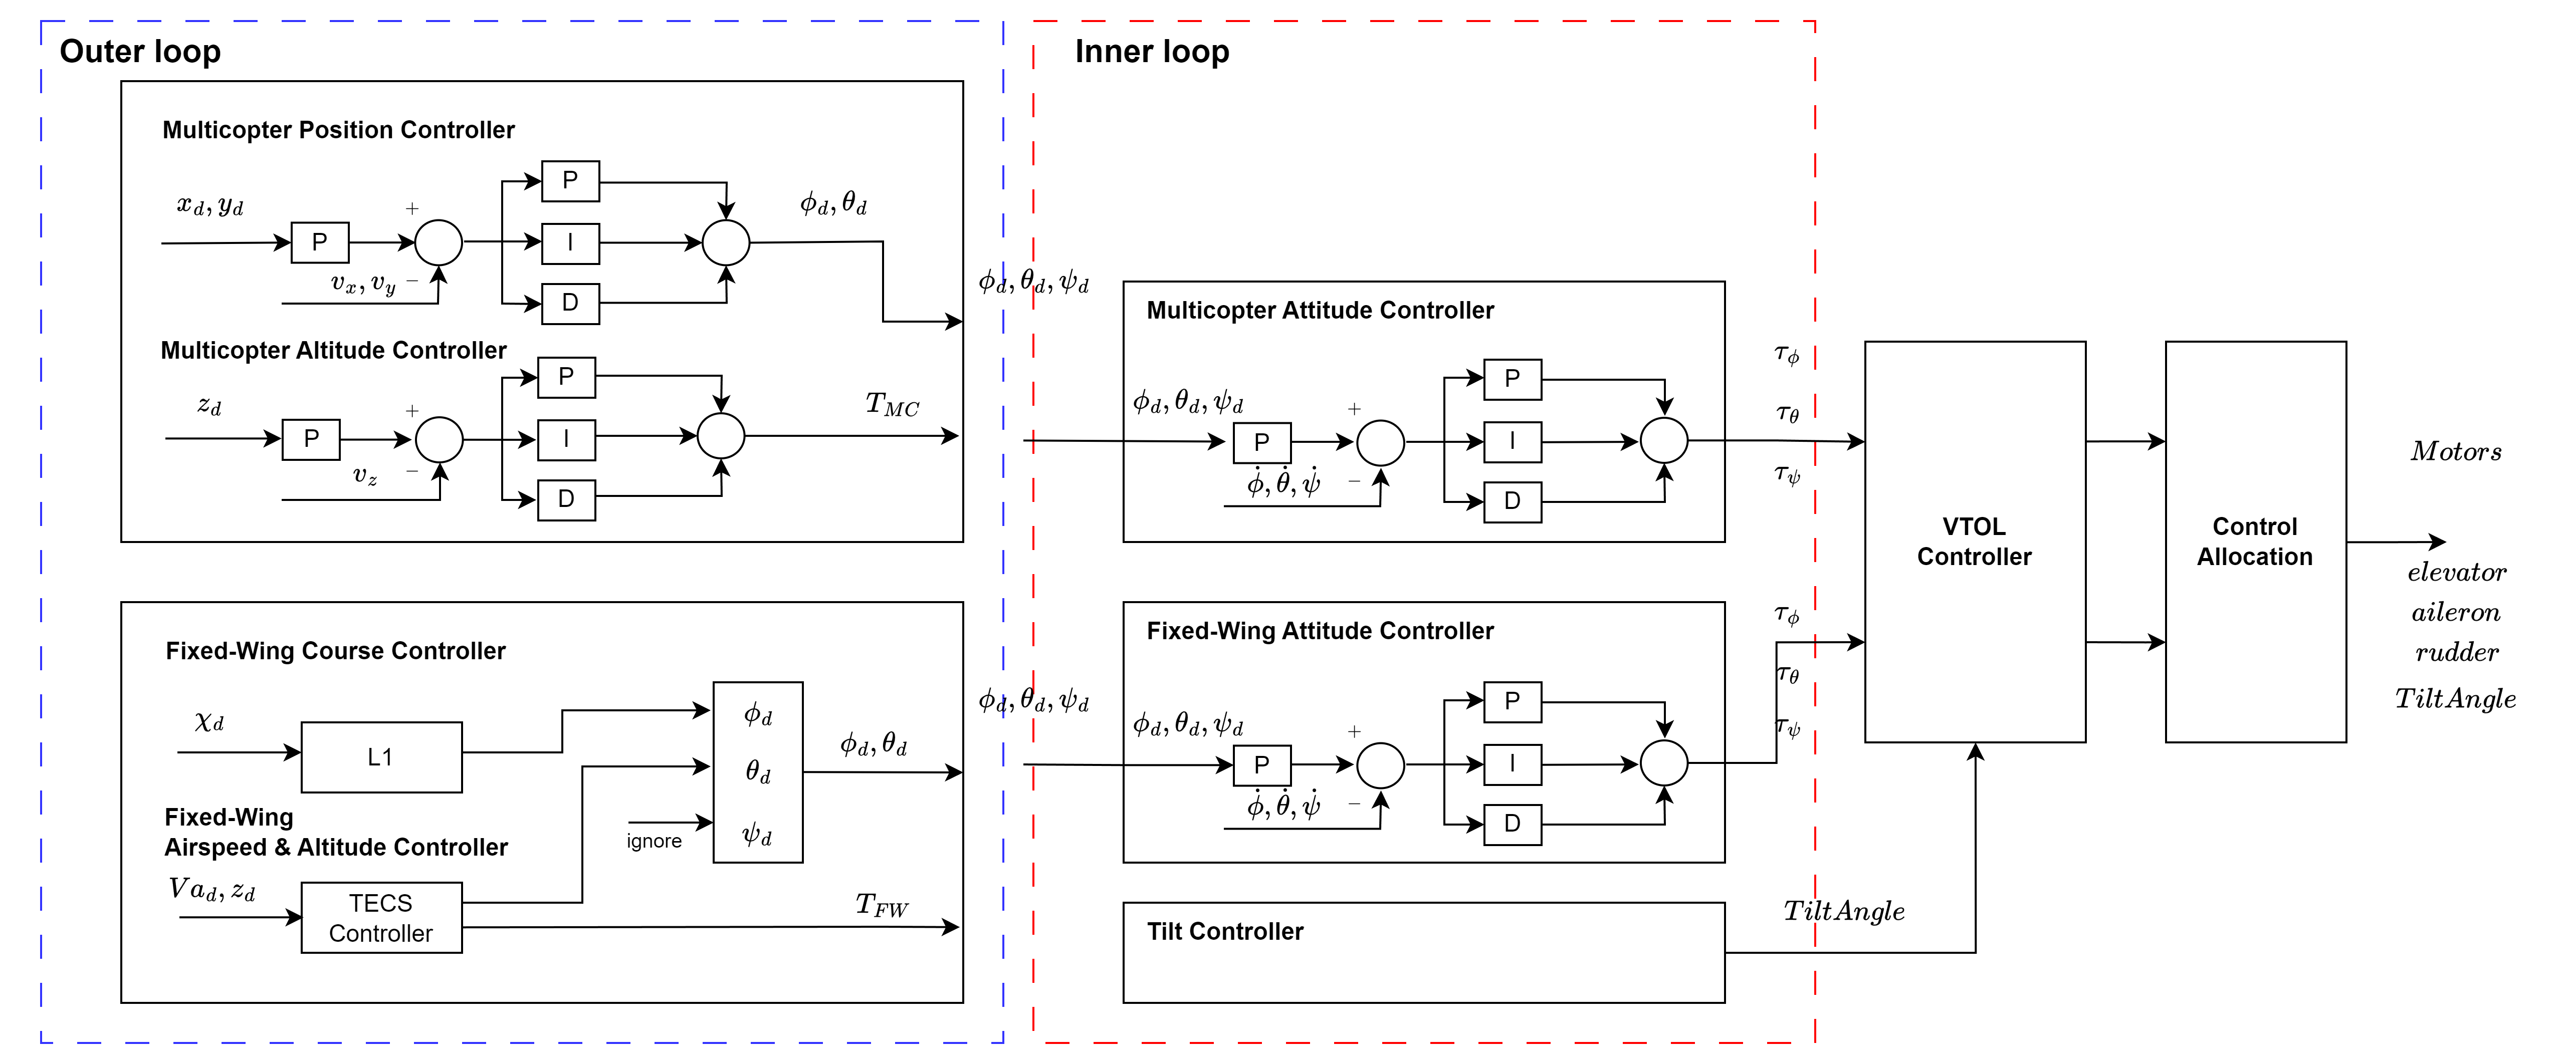
\includegraphics[width=1\linewidth]{PX4_VTOL_Control_Structure.png}
    \caption{PX4 VTOL Control Structure}
    \label{fig:enter-label}
\end{figure}
%%%%%%%%%%%%%%%%%%%%%%%%%%%%%%%%%%%%%%%%%%
% Section 2
\section{Literature Review}
\subsection{Analysis of Open-Source Autopilot Transition Phase}
Open-source autopilot systems, such as PX4, support a variety of unmanned aerial vehicles (UAVs), including tiltrotor eVTOLs. However, their transition logic from hover to forward flight relies on simplified strategies that inadequately address the complex dynamics of hybrid aircraft.

\subsubsection{Transition Phase Operation}
The transition phase in open-source autopilots involves two key mechanisms:
\begin{itemize}
    \item \text{Open Loop Tilt Angle Control} \\
    The front rotor of the tilt rotor tilts to a certain angle to achieve airspeed during the transition. Once the transition starting speed (BLENDED\_ASPD) is reached, the transition algorithm begins. Until transition completion airspeed, tilt angle keep particular tilt angle(VT\_TILT\_TRANS). When the transition completion speed (TRANSITION\_ASPD) is reached, the switch to fixed-wing mode starts.
    \item \text{Linear Weighting of Control Outputs} \\
    At this point, the outputs for attitude control of the fixed-wing and rotary-wing are divided based on the current airspeed with weighting applied. Once the transition completion speed (TRANSITION\_ASPD) is reached, the output of the fixed-wing control takes over completely.
\end{itemize}

\begin{center}
    \begin{tikzpicture}[
       node distance=1.8cm and 2cm,
       every node/.style={font=\small},
       box/.style={draw, rectangle, rounded corners, minimum width=4cm, minimum height=1cm, align=center},
       arrow/.style={-{Latex}, thick}
       ]
       
       \node (label) at (0, 0) {Transition Start};
       
       \node[draw, diamond, aspect=2, minimum width=3.5cm, align=center, below=of label] (cond1) {$V_a \ge \text{Blended\_Aspd}$};
       
       \node[draw, diamond, aspect=2, minimum width=3.5cm, align=center, below=of cond1] (cond2) {$V_a \ge \text{Transition\_Aspd}$};
       
       \node[draw, diamond, aspect=2, minimum width=3.5cm, align=center, below=of cond2] (cond3) {$V_a \ge \text{Transition\_Aspd}$};
       
       
       \node[below=of cond3] (next) {Transition Completed};
       
       \draw[arrow] (label) -- node[right, yshift=-11pt, align=left]{
          $\delta_c = \text{tilt forward angle} = 15^\circ$
       } (cond1);
       
       \draw[arrow] (cond1) -- node[right, yshift=0pt, align=left]{
          True \\
          ~ \\
          ~ \\
          $\delta_c = \text{critical tilt angle} = 45^\circ$
       } (cond2);
       
       \draw[arrow] (cond2) -- node[right, yshift=0pt, align=left]{
          True \\
          ~ \\
          ~ \\
          $\delta_c = \text{tilt angle} = 90^\circ$
       }  (cond3);
       
       \draw[arrow] (cond3) -- node[right, yshift=2pt]{True} (next);
       
       \draw[arrow] (cond1.west) -- ++(-1.315, 0) -- (-3.35, -1.1) -- (0, -1.1);
       \node at ([xshift=-2.5cm,yshift=-0.2cm]cond1.north) {False};
       
       \draw[arrow] (cond2.west) -- ++(-1.11, 0) -- (-3.3, -4.9) -- (0, -4.9);
       \node at ([xshift=-2.5cm,yshift=-0.2cm]cond2.north) {False};
       
       \draw[arrow] (cond3.west) -- ++(-1.11, 0) -- (-3.3, -8.9) -- (0, -8.9);
       \node at ([xshift=-2.5cm,yshift=-0.2cm]cond3.north) {False};
       
       \coordinate (padUL1) at ($(label.north west) + (-2.5, 0.0)$);
       \coordinate (padLR1) at ($(cond1.south east) + (3.2, -0.5)$);
       \node[draw=black, dashed, rounded corners, fit=(padUL1)(padLR1)] {};
       \node[anchor=north east, font=\bfseries] at ($(padLR1) + (0.0, 4.2)$) {MC Mode};
       
       \coordinate (padUL2) at ($(cond2.north west) + (-2.67, 2.07)$);
       \coordinate (padLR2) at ($(cond3.south east) + (3.15, -0.5)$);
       \node[draw=black, dashed, rounded corners, fit=(padUL2)(padLR2)] {};
       \node[anchor=north east, font=\bfseries] at ($(padLR2) + (0.0, 7.65)$) {Transition};
       
       \coordinate (padUL3) at ($(next.north west) + (-2.08, 1.55)$);
       \coordinate (padLR3) at ($(next.south east) + (2.58, -0.0)$);
       \node[draw=black, dashed, rounded corners, fit=(padUL3)(padLR3)] {};
       \node[anchor=north east, font=\bfseries] at ($(padLR3) + (-0.0, 2.1)$) {FW Mode};
       
    \end{tikzpicture}
 \end{center}


In the transition phase, the autopilot does not consider the aircraft's nonlinear dynamics, such as rotor tilt angle changes, which can lead to altitude loss and instability post-transition.

\subsection{Total Energy Control System (TECS)}
The Total Energy Control System (TECS) is a control strategy used in aircraft to manage their total energy, which consists of potential energy (\(E_P = mgh\)) and kinetic energy (\(E_K = \frac{1}{2}mv^2\)). TECS regulates airspeed and altitude by coordinating throttle and pitch inputs: throttle adjusts the total energy, while pitch controls the distribution of energy between altitude and speed.

\begin{figure}[H]
    \centering
    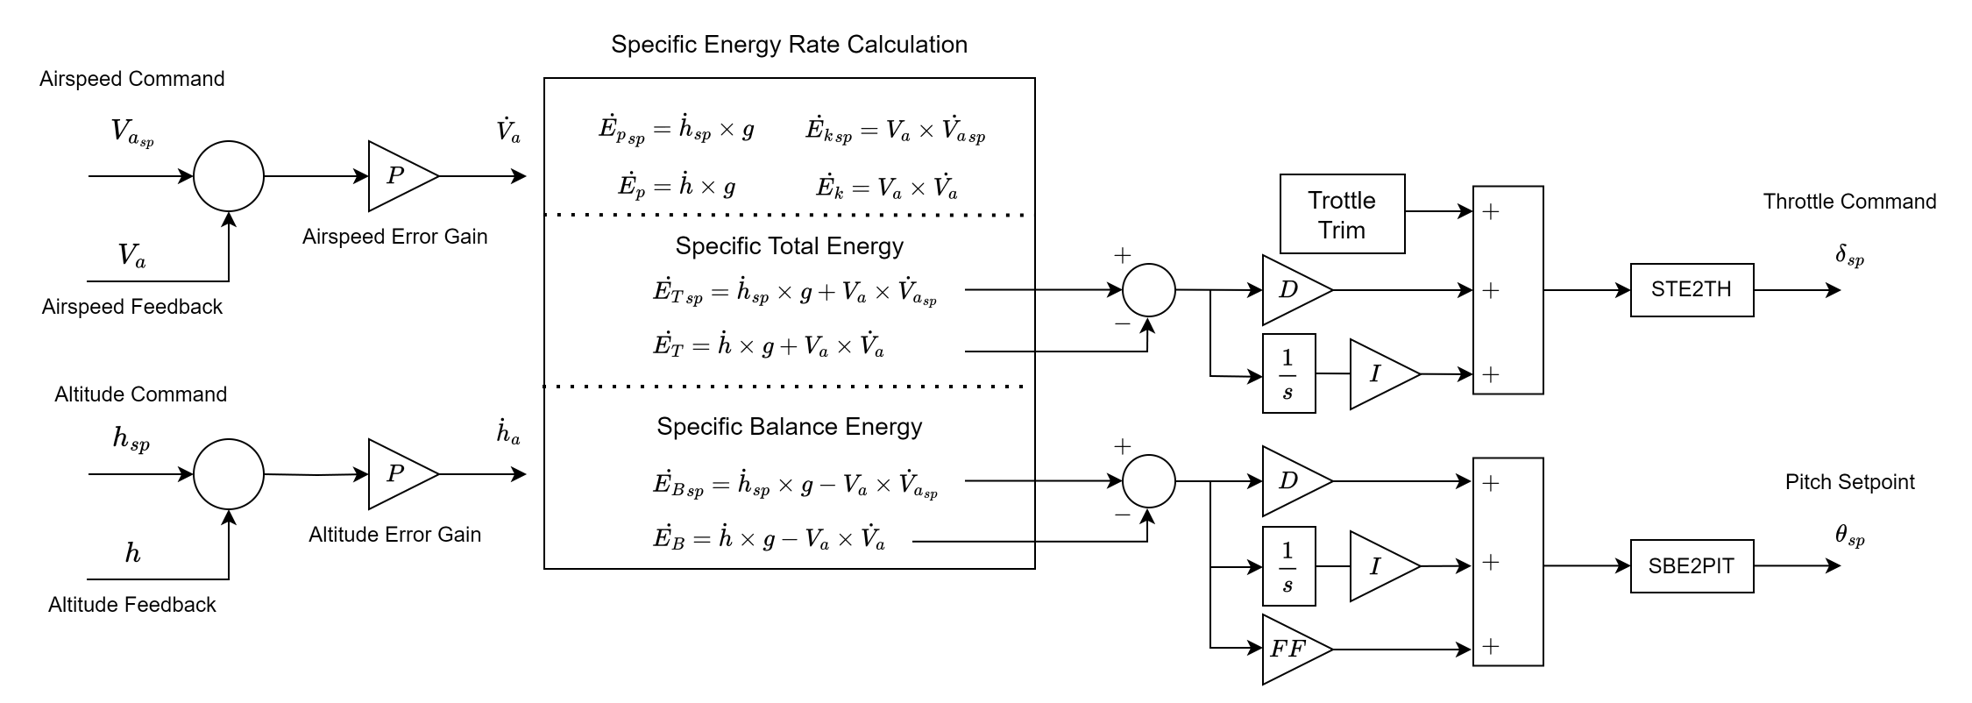
\includegraphics[width=1\linewidth]{PX4_TECS_Structure.png}
    \caption{PX4 TECS Control Structure}
    \label{fig:enter-label}
\end{figure}
In the Open-Source autopilot framework, TECS remains inactive during the transition phase of tiltrotor eVTOLs and only activates once the aircraft fully enters fixed-wing mode.

\subsubsection{TECS Control Structure}
TECS manages two primary functions:
\begin{itemize}
    \item \text{Total Energy Control}: Adjusts throttle to regulate the total specific energy rate (\(\dot{E}_T = \dot{E}_P + \dot{E}_K\)), where:
    \begin{itemize}
        \item \(\dot{E}_P = \dot{h}g\) (potential energy rate, linked to altitude change),
        \item \(\dot{E}_K = v\dot{v}\) (kinetic energy rate, linked to speed change).
    \end{itemize}
    \item \text{Balance Energy Control}: Adjusts pitch to control the balance specific energy rate (\(\dot{E}_B = \dot{E}_P - \dot{E}_K\)), ensuring proper energy distribution between altitude and airspeed.
\end{itemize}

The setpoints for these energy rates are defined as:
\begin{equation}
    \dot{E}_{T_{\text{sp}}} = \dot{h}_{\text{sp}}g + v_a\dot{v}_{a_{\text{sp}}}, \quad \dot{E}_{B_{\text{sp}}} = \dot{h}_{\text{sp}}g - v_a\dot{v}_{a_{\text{sp}}}
\end{equation}
where \(\dot{h}_{\text{sp}}\) is the desired altitude rate, \(v_a\) is the current airspeed, and \(\dot{v}_{a_{\text{sp}}}\) is the desired airspeed rate.

The control outputs—thrust (\(\delta_{\text{sp}}\)) and pitch (\(\theta_{\text{sp}}\))—are calculated as:
\begin{equation}
    \delta_{\text{sp}} = \left( D_T (\dot{E}_{T_{\text{sp}}} - \dot{E}_T) + I_T \int (\dot{E}_{T_{\text{sp}}} - \dot{E}_T) \, dt + T_{\text{cruise}} \right) \frac{1}{\dot{E}_{T,\text{max}} - \dot{E}_{T,\text{min}}}
\end{equation}
\begin{equation}
    \theta_{\text{sp}} = \left( D_B (\dot{E}_{B_{\text{sp}}} - \dot{E}_B) + I_B \int (\dot{E}_{B_{\text{sp}}} - \dot{E}_B) \, dt + ff_B \dot{E}_{B_{\text{sp}}} \right) \frac{1}{v_a g}
\end{equation}
where:
\begin{itemize}
    \item \(D_T, I_T\): Derivative and integral gains for specific total energy rate,
    \item \(D_B, I_B\): Derivative and integral gains for specific balance energy rate,
    \item \(ff_B\): Feedforward gain,
    \item \(T_{\text{cruise}}\): Cruise thrust,
    \item \(\dot{E}_{T,\text{max}} = g \times \text{max\_climb\_rate}\), \(\dot{E}_{T,\text{min}} = g \times \text{max\_descent\_rate}\): Limits on energy rates.
\end{itemize}

For tiltrotors, the transition phase introduces unique dynamics, such as rotor tilt angle changes, which affect the balance between \(\dot{E}_P\) and \(\dot{E}_K\). Fixed gains, as used in PX4’s default TECS, fail to adapt to these rapid changes, resulting in delayed altitude recovery and instability post-transition.

\section{Methodology}
\subsection{Neural Network-Based Gain Tuning Methodology}
To overcome the limitations of static TECS gains, this study proposes a neural network-based approach for real-time gain tuning, specifically tailored to the post-transition phase of tiltrotor eVTOLs. The methodology dynamically adjusts the proportional (\(K_p\)) and integral (\(K_i\)) gains of TECS based on the aircraft’s flight state, mitigating altitude loss and improving stability immediately after the transition to fixed-wing mode.

\subsubsection{Why Use a Neural Network?}
Immediately after the transition to fixed-wing mode, the aircraft experiences residual effects from the transition phase, such as aerodynamic shifts and thrust vector changes. Fixed gains cannot adequately respond to these variations, leading to poor altitude control. A neural network enables real-time adaptation by learning and adjusting gains based on current errors (e.g., altitude and energy rate deviations), offering a robust solution for open-source platforms like PX4.

\subsubsection{Neural Network Design}
The proposed neural network is a simple two-layer feedforward network:
\begin{itemize}
    \item \textbf{Inputs}:
    \begin{itemize}
        \item Proportional error: \(e_p(k) = \dot{E}_{\text{sp}}(k) - \dot{E}(k)\),
        \item Integral error: \(e_i(k) = \sum \int e_p(k) \, dt\).
    \end{itemize}
    \item \textbf{Outputs}:
    \begin{itemize}
        \item Adjusted gains \(K_p(k)\) and \(K_i(k)\), computed using a sigmoid activation function:
        \begin{equation}
            f(x) = \frac{2(1 - e^{-x \cdot Y_g})}{Y_g (1 + e^{-x \cdot Y_g})}
        \end{equation}
        where \(x(k) = K_p(k)e_p(k) + K_i(k)e_i(k)\), and \(Y_g\) is a tuning parameter shaping the sigmoid curve in figure \ref{fig:sigmoid_function_shapes}.
    \end{itemize}
\end{itemize}

The control input \(u(k) = f(x)\) drives the TECS outputs (thrust and pitch), with gains updated dynamically.

\begin{figure}[H]
    \centering
    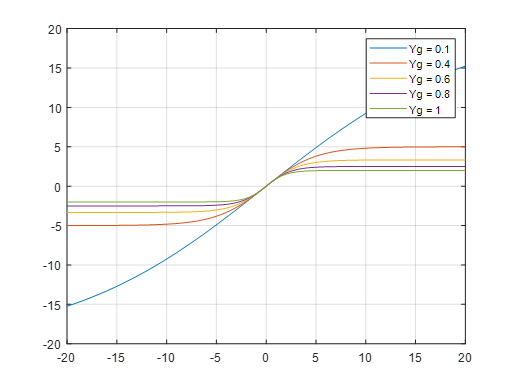
\includegraphics[width=0.6\linewidth]{sigmoid_function_shapes.png}
    \caption{Sigmoid function shapes for different \(Y_g\) values}
    \label{fig:sigmoid_function_shapes}
\end{figure}

\begin{figure}[H]
    \centering
    
\includegraphics[width=0.6\linewidth]{neural_network_diagram.png}
    \caption{Neural network block diagram for adaptive TECS gain tuning}
    \label{fig:neural_network_block_diagram}
\end{figure}

\subsection{Tuning Process}
The gains are tuned using the steepest descent method to minimize the cost function:
\begin{equation}
    J(k) = \frac{1}{2}(\dot{E}_{\text{sp}}(k) - \dot{E}(k))^2
\end{equation}

The update rules are:
\begin{equation}
    K_p(k+1) = K_p(k) - \eta_p \frac{\partial J(k)}{\partial K_p(k)}, \quad K_i(k+1) = K_i(k) - \eta_i \frac{\partial J(k)}{\partial K_i(k)}
\end{equation}
with partial derivatives:
\begin{equation}
    \frac{\partial J(k)}{\partial K_p(k)} = -e_p(k) \cdot f'(x(k)) \cdot e_p(k), \quad \frac{\partial J(k)}{\partial K_i(k)} = -e_p(k) \cdot f'(x(k)) \cdot e_i(k)
\end{equation}
where \(f'(x) = \frac{4e^{-x \cdot Y_g}}{(1 + e^{-x \cdot Y_g})^2}\), and \(\eta_p\), \(\eta_i\) are learning rates.

This method replaces static gains with a dynamic, state-dependent tuning mechanism, ensuring computational efficiency for real-time implementation on autopilot systems.


\subsection{Implementation and Validation}
The proposed method will be implemented and tested using PX4 simulations, focusing on the post-transition phase in fixed-wing mode. Performance will be evaluated by comparing altitude stability and recovery time against the default fixed-gain TECS.


\section{Model}
\subsection{Aircraft Model}
In simulation, we focus on longitudinal dynamics, including altitude, airspeed, and pitch attitude control. The aircraft model used in the simulation is a tiltrotor eVTOL with the following parameters:
% \begin{table}[H]
%     \caption{Aircraft Model Parameters}
%     \label{tab:aircraft_model_parameters}
%     \small
%     \begin{tabular}{|l|c|c|}
%     \hline
%     \textbf{Parameter} & \textbf{Symbol} & \textbf{Value} \\ \hline
    
%     \multicolumn{3}{|c|}{\textbf{Physical Properties}} \\ \hline
%     Mass & \( m \) & 5.22 kg \\ \hline
%     Inertia (\( J_x \)) & \( J_x \) & 1.229 kg·m² \\ \hline
%     Inertia (\( J_y \)) & \( J_y \) & 0.1702 kg·m² \\ \hline
%     Inertia (\( J_z \)) & \( J_z \) & 0.8808 kg·m² \\ \hline
%     Inertia (\( J_{xz} \)) & \( J_{xz} \) & 0.9343 kg·m² \\ \hline
%     Wing Area & \( S_{\text{wing}} \) & 0.75 m² \\ \hline
%     Wing Span & \( b \) & 2.10 m \\ \hline
%     Mean Aerodynamic Chord & \( c \) & 0.3571 m \\ \hline
    
%     \multicolumn{3}{|c|}{\textbf{Aerodynamic Coefficients}} \\ \hline
%     Lift Coefficient (zero angle) & \( C_{L_0} \) & 0.0867 \\ \hline
%     Lift Coefficient (alpha) & \( C_{L_\alpha} \) & 4.02 \\ \hline
%     Lift Coefficient (q) & \( C_{L_q} \) & 3.8954 \\ \hline
%     Lift Coefficient (delta\_e) & \( C_{L_{\delta_e}} \) & 0.278 \\ \hline
%     Drag Coefficient (zero angle) & \( C_{D_0} \) & 0.0197 \\ \hline
%     Drag Coefficient (alpha) & \( C_{D_\alpha} \) & 0.0791 \\ \hline
%     Drag Coefficient (alpha²) & \( C_{D_{\alpha^2}} \) & 1.06 \\ \hline
%     Drag Coefficient (q) & \( C_{D_q} \) & 0.0 \\ \hline
%     Drag Coefficient (delta\_e) & \( C_{D_{\delta_e}} \) & 0.0633 \\ \hline
%     Moment Coefficient (zero angle) & \( C_{m_0} \) & 0.0302 \\ \hline
%     Moment Coefficient (alpha) & \( C_{m_\alpha} \) & -0.126 \\ \hline
%     Moment Coefficient (q) & \( C_{m_q} \) & -1.3047 \\ \hline
%     Moment Coefficient (delta\_e) & \( C_{m_{\delta_e}} \) & -0.206 \\ \hline

%     \end{tabular}
% \end{table}

\begin{figure}[H]
    \centering
    \begin{minipage}{0.45\linewidth}
        \centering
        \begin{tabular}{|l|c|}
            \hline            
            \multicolumn{2}{|c|}{\textbf{Physical Properties}} \\ \hline
            \textbf{Symbol} & \textbf{Value} \\ \hline
            \( m \) & 5.22 kg \\ \hline
            \( J_x \) & 1.229 kg·m² \\ \hline
            \( J_y \) & 0.1702 kg·m² \\ \hline
            \( J_z \) & 0.8808 kg·m² \\ \hline
            \( J_{xz} \) & 0.9343 kg·m² \\ \hline
            \( S_{\text{wing}} \) & 0.75 m² \\ \hline
            \( b \) & 2.10 m \\ \hline
            \( \bar{c} \) & 0.3571 m \\ \hline
        \end{tabular}
        \vspace{0.5em} % 표와 캡션 사이의 여백 추가
        \captionof{table}{Physical Properties}
        \label{tab:aircraft_model_parameters}
    \end{minipage}
    \hfill % 표와 그림 사이에 여백 추가
    \begin{minipage}{0.45\linewidth}
        \centering
        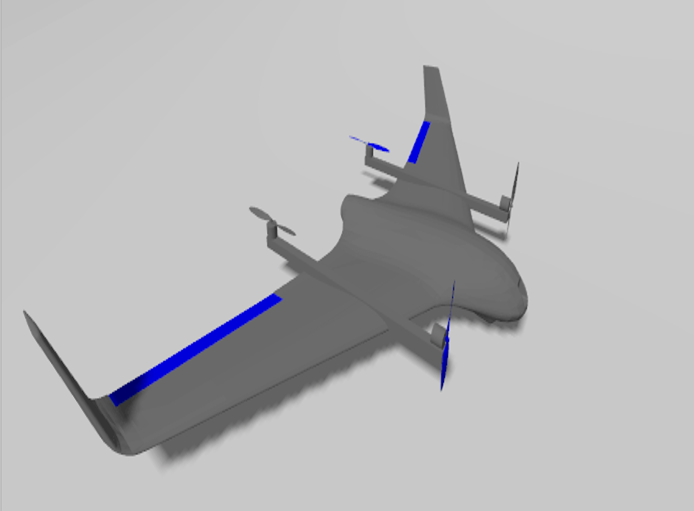
\includegraphics[width=\linewidth]{tiltrotor_gazebo.png}
        \captionof{figure}{Tiltrotor Gazebo model}
        \label{fig:tiltrotor_gazebo}
    \end{minipage}
    \caption{Aircraft Model Parameters and Tiltrotor Gazebo Model}
    \label{fig:aircraft_model_parameters_and_gazebo}
\end{figure}

where \(m\) is the mass, \(J_x, J_y, J_z, J_{xz}\) are the moments of inertia, \(S_{\text{wing}}\) is the wing area, \(b\) is the wing span, and \(\bar{c}\) is the mean aerodynamic chord. The aerodynamic coefficients are also provided in Table \ref{tab:aircraft_model_parameters}.

\begin{table}[H]
    \centering
    \label{tab:aero_coefficients}
    % 공통 제목
    \textbf{Aerodynamic Coefficients} \\ % 공통 제목을 tabular 밖에서 텍스트로
    \vspace{0.5cm} % 제목과 표 사이 간격 조정
    \begin{adjustbox}{valign=t}
    \begin{minipage}[t]{0.45\textwidth} % [t]로 위쪽 정렬
        \centering
        \begin{tabular}{|l|c|}
            \hline
            \textbf{Symbol} & \textbf{Value} \\ \hline
            \( C_{L_0} \) & 0.0867 \\ \hline
            \( C_{L_\alpha} \) & 4.02 \\ \hline
            \( C_{L_q} \) & 3.8954 \\ \hline
            \( C_{L_{\delta_e}} \) & 0.278 \\ \hline
            \( C_{D_0} \) & 0.0197 \\ \hline
            \( C_{D_\alpha} \) & 0.0791 \\ \hline
            \( C_{D_{\alpha^2}} \) & 1.06 \\ \hline
        \end{tabular}
    \end{minipage}
    \end{adjustbox}
    \hfill
    \begin{adjustbox}{valign=t}
    \begin{minipage}[t]{0.45\textwidth} % [t]로 위쪽 정렬
        \centering
        \begin{tabular}{|l|c|}
            \hline
            \textbf{Symbol} & \textbf{Value} \\ \hline
            \( C_{D_q} \) & 0.0 \\ \hline
            \( C_{D_{\delta_e}} \) & 0.0633 \\ \hline
            \( C_{m_0} \) & 0.0302 \\ \hline
            \( C_{m_\alpha} \) & -0.126 \\ \hline
            \( C_{m_q} \) & -1.3047 \\ \hline
            \( C_{m_{\delta_e}} \) & -0.206 \\ \hline
            \( \) & \( \) \\ \hline % 높이 맞추기 위해 빈 행 추가
        \end{tabular}
    \end{minipage}
    \end{adjustbox}
    \caption{Aerodynamic Coefficients of the Aircraft Model}
\end{table}
The aerodynamic coefficients are provided in Table \ref{tab:aircraft_model_parameters}. The lift, drag, and moment coefficients are defined as:

where \(C_{L_0}\) is the lift coefficient at zero angle of attack, \(C_{L_\alpha}\) is the lift coefficient per unit angle of attack, \(C_{L_q}\) is the lift coefficient per unit pitch rate, \(C_{L_{\delta_e}}\) is the lift coefficient per unit elevator deflection, \(C_{D_0}\) is the drag coefficient at zero angle of attack, \(C_{D_\alpha}\) is the drag coefficient per unit angle of attack, \(C_{D_{\alpha^2}}\) is the drag coefficient per unit angle of attack squared, \(C_{D_q}\) is the drag coefficient per unit pitch rate, \(C_{D_{\delta_e}}\) is the drag coefficient per unit elevator deflection, \(C_{m_0}\) is the moment coefficient at zero angle of attack, \(C_{m_\alpha}\) is the moment coefficient per unit angle of attack, \(C_{m_q}\) is the moment coefficient per unit pitch rate, and \(C_{m_{\delta_e}}\) is the moment coefficient per unit elevator deflection.
\begin{equation}
    L = \frac{1}{2} \rho v^2 S C_L, \quad D = \frac{1}{2} \rho v^2 S C_D, \quad M = \frac{1}{2} \rho v^2 S C_m
\end{equation}
where \(L\) is the lift force, \(D\) is the drag force, \(M\) is the moment, \(\rho\) is the air density, \(v\) is the airspeed, and \(S\) is the wing area.


\subsection{Control System}
The control system for the tiltrotor eVTOL consists of the following components:
\begin{itemize}
    \item \textbf{Multicopter Attitude Control}: PID controllers for roll, pitch, and yaw control in Multicopter mode.
    \item \textbf{Multicopter Altitude Control}: PID controller for altitude control in Multicopter mode.
    \item \textbf{Fixed-Wing Attitude Control}: PID controller for attitude control in Fixed-Wing mode.
    \item \textbf{TECS}: Total Energy Control System for airspeed and altitude regulation.
\end{itemize}

\begin{figure}[H]
    \centering
    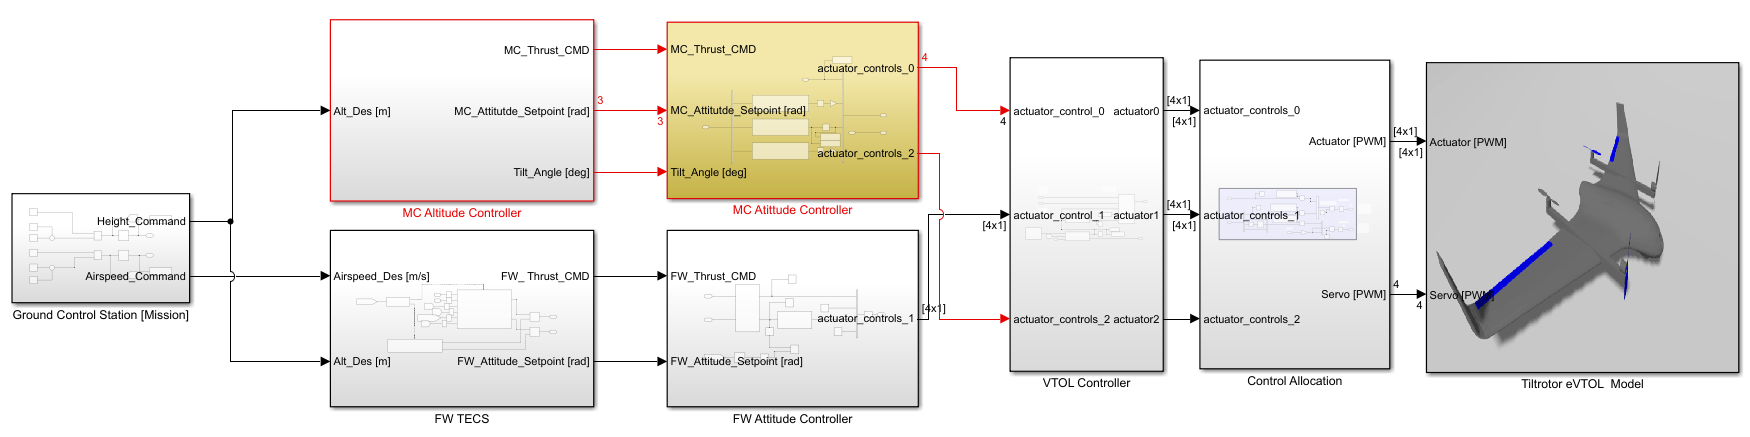
\includegraphics[width=0.8\linewidth]{control_system_diagram.png}
    \caption{Control System Diagram}
    \label{fig:control_system_diagram}
\end{figure}

The control system diagram is shown in Figure \ref{fig:control_system_diagram}.

In simulation, we focus on longitudinal dynamics, including altitude, airspeed, and pitch attitude control. 



%%%%%%%%%%%%%%%%%%%%%%%%%%%%%%%%%%%%%%%%%%
\section{Simulation Results}
The proposed neural network-based adaptive TECS gain tuning method was implemented in PX4 simulations to evaluate its performance during the post-transition phase of a tiltrotor eVTOL. The results were compared against the default fixed-gain TECS configuration to assess improvements in altitude stability and recovery time.

\subsection{Simulation Setup}
The simulation environment used MATLAB Simulink. The aircraft model was integrated with the neural network-based adaptive TECS gain tuning method, replacing the default fixed gains. The simulation focused on the post-transition phase, with the aircraft transitioning to fixed-wing mode at a predetermined airspeed. The initial condition is from the transition phase, so we consider some parameters in the transition phase to set the condition of transition. The parameters that influence the transition performance are:

\begin{itemize}
    \item \text{BLENDED\_ASPD}: The airspeed at which the transition from multicopter mode to blended mode begins.
    \item \text{TRANSITION\_ASPD}: The airspeed at which the transition to fixed-wing mode is completed.
    \item \text{TILT\_RATE}: The rate at which the rotors tilt during the transition phase.
\end{itemize}

These parameters are critical in determining the smoothness and stability of the transition phase. For the simulation, the following values were used:
\begin{itemize}
    \item BLENDED\_ASPD = 10 m/s
    \item TRANSITION\_ASPD = 15 m/s
    \item TILT\_RATE = 15 deg/s
\end{itemize}

\subsection{TECS State Response}
Figure \ref{fig:tecs_state_response} show the altitude and airspeed responses across the entire simulation period (0-100 sec), respectively. The neural network-based TECS demonstrates significantly faster altitude recovery compared to the PX4 fixed-gain TECS, while both methods exhibit similar airspeed stabilization.

\begin{figure}[H]
    \centering
    \begin{minipage}{0.45\textwidth}
        \centering
        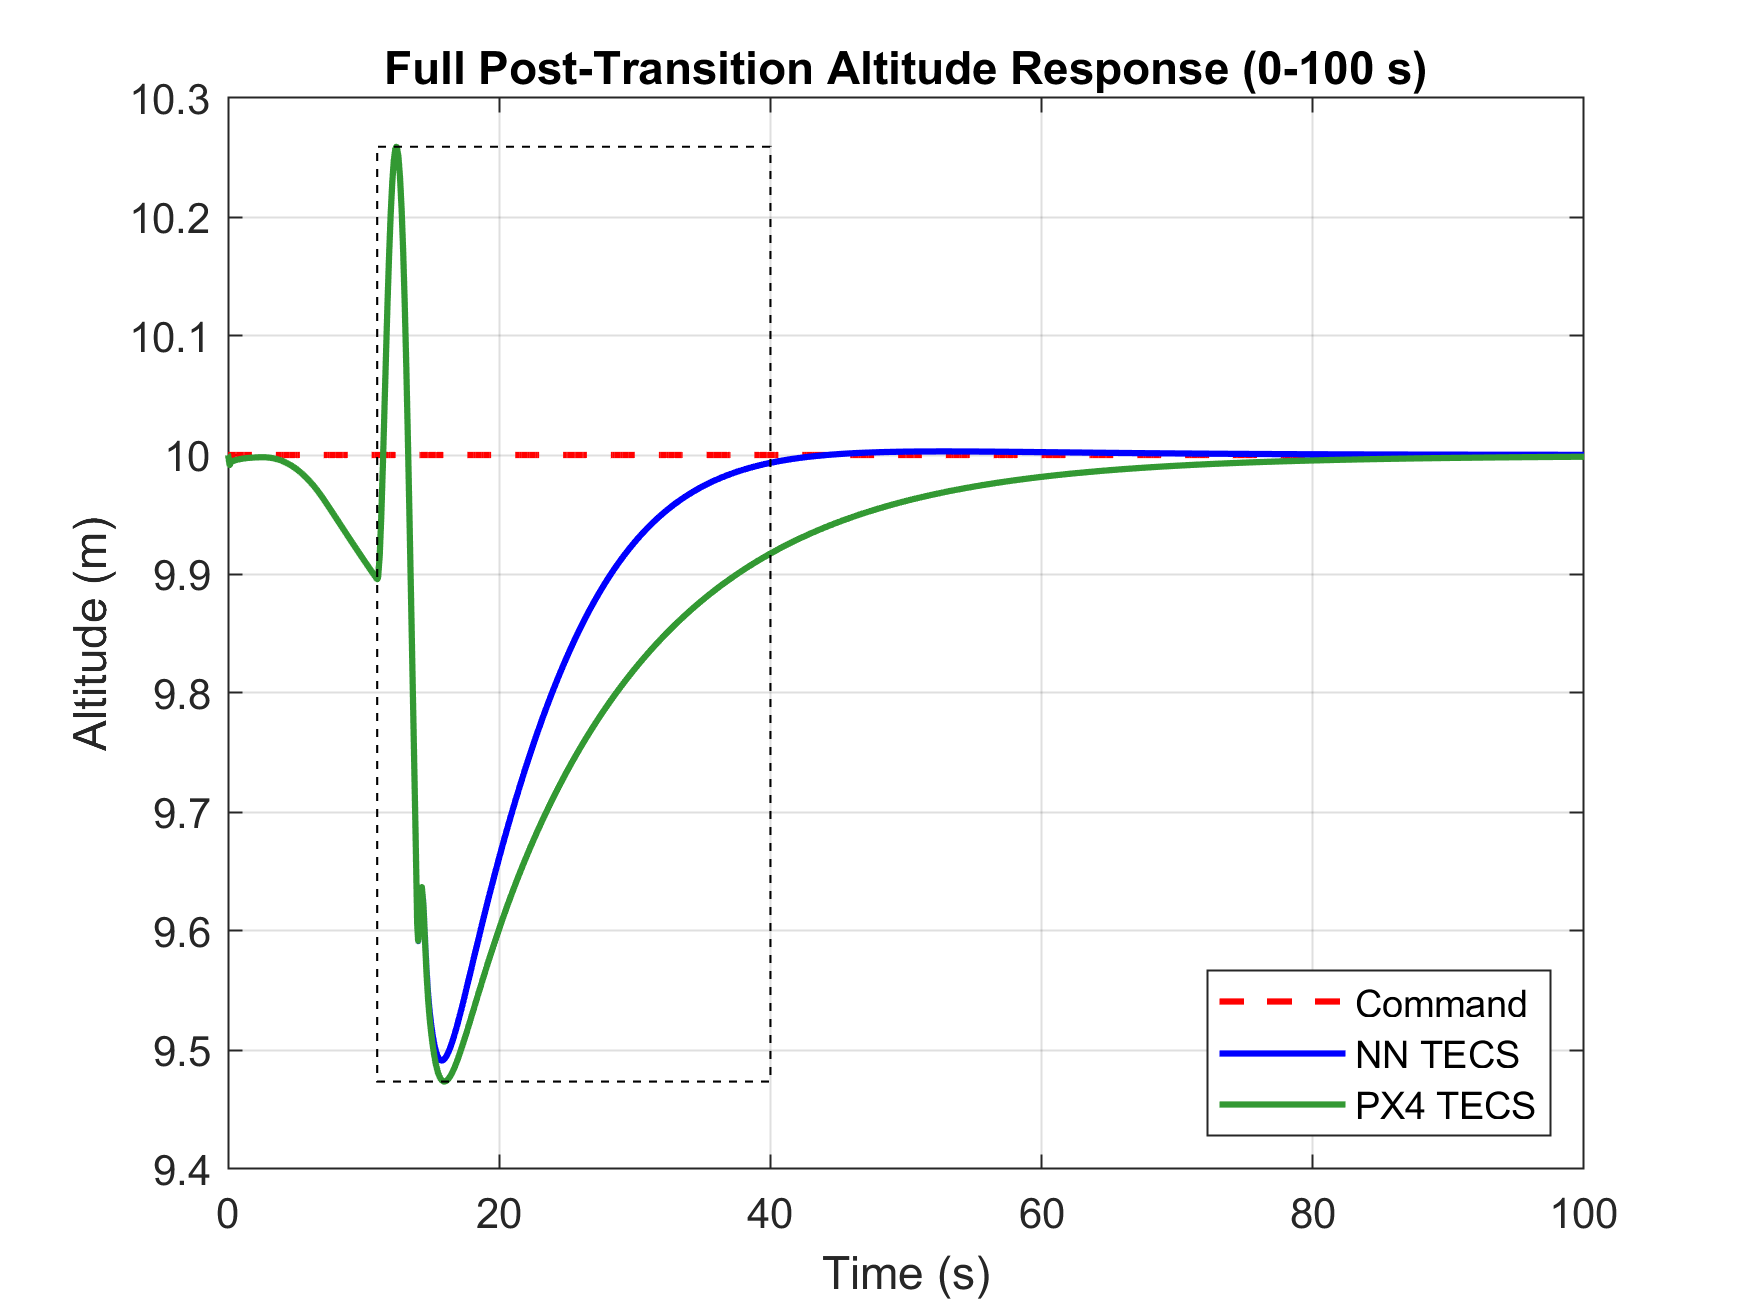
\includegraphics[width=\linewidth]{full_altitude_plot.png}
    \end{minipage}
    \hfill
    \begin{minipage}{0.45\textwidth}
        \centering
        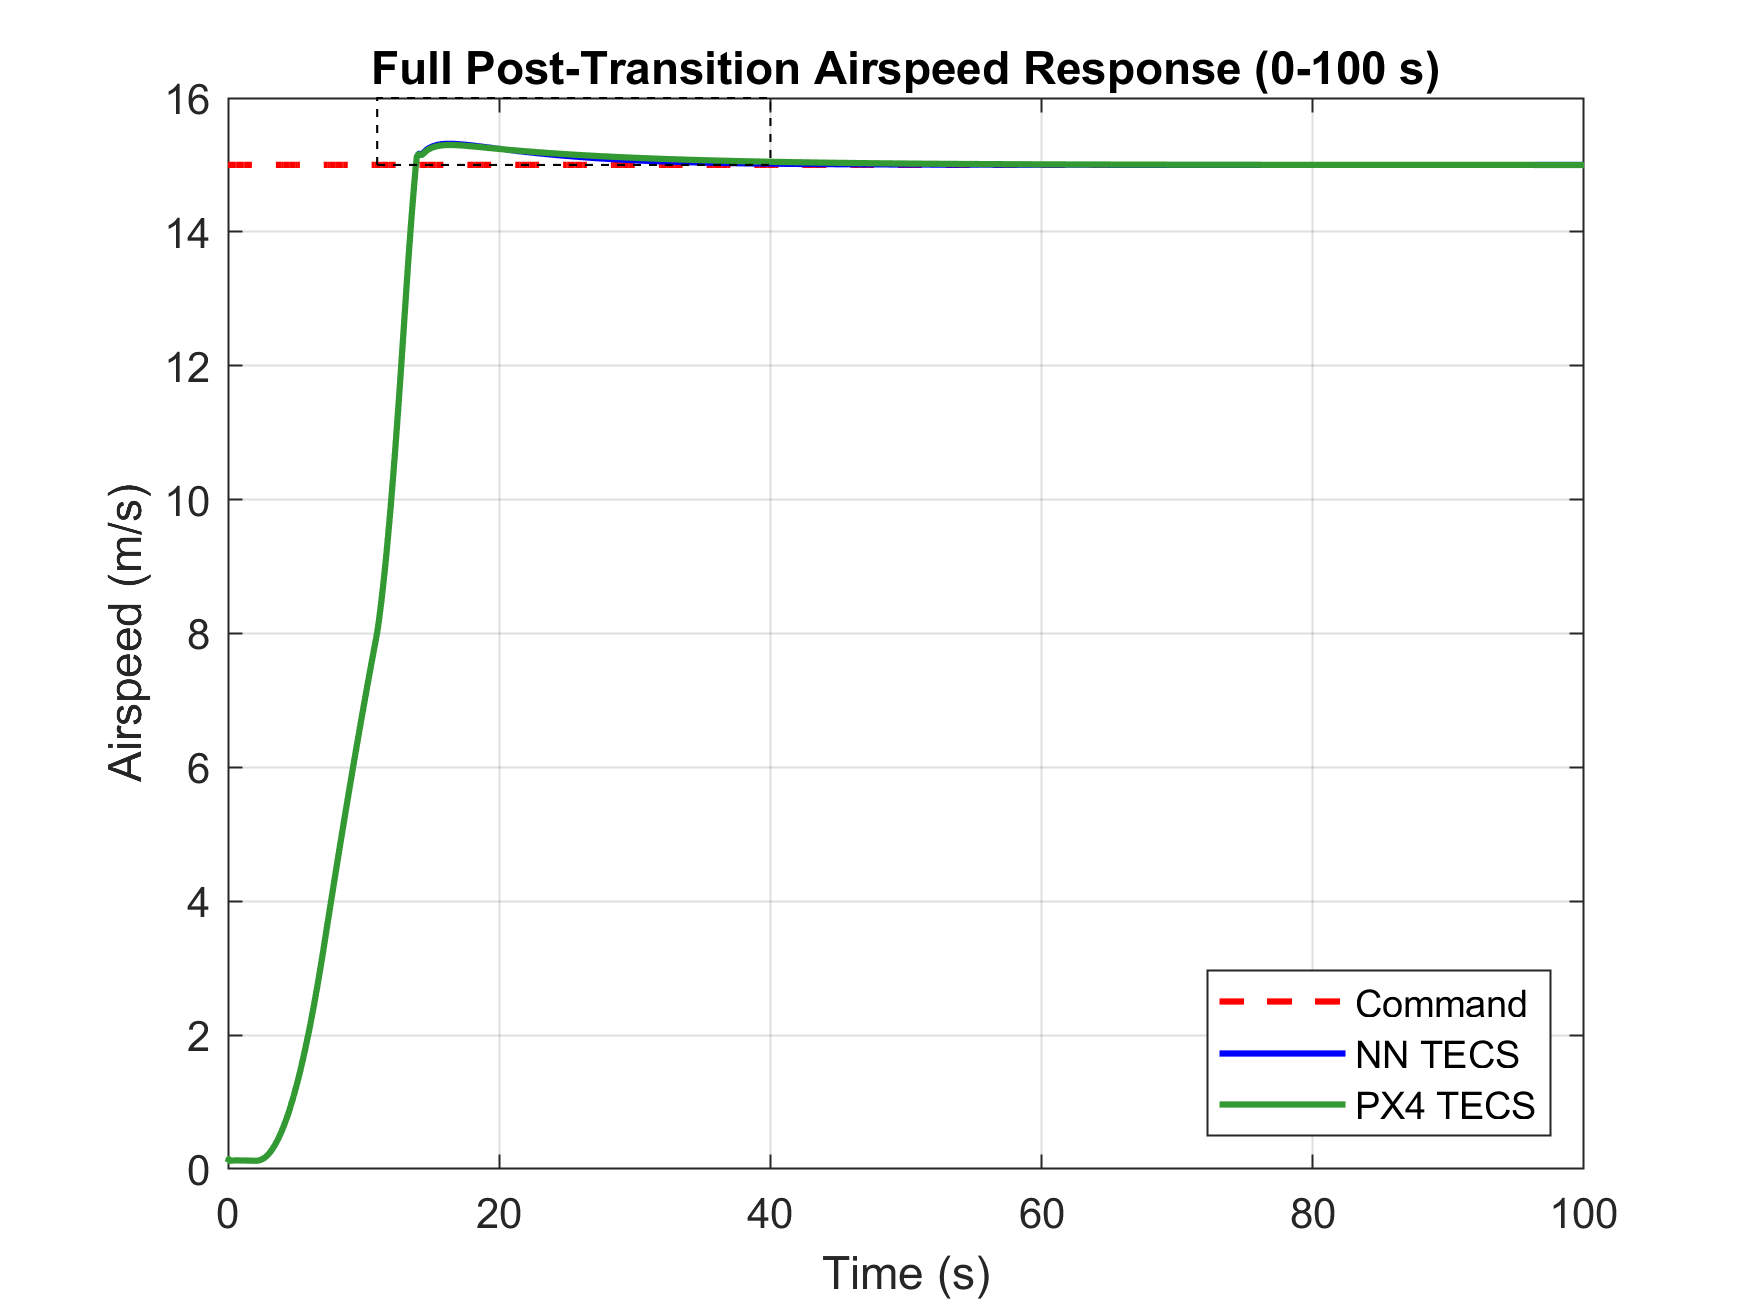
\includegraphics[width=\linewidth]{full_airspeed_plot.png}
    \end{minipage}
    \caption{TECS State Response: Altitude and Airspeed Comparison.}
    \label{fig:tecs_state_response}
\end{figure}

\subsection{Flight Mode}
In Figure \ref{fig:flight_state}, we illustrate the transition from multicopter mode to fixed-wing mode, where TECS is activated in fixed-wing mode.

\begin{figure}[H]
    \centering
    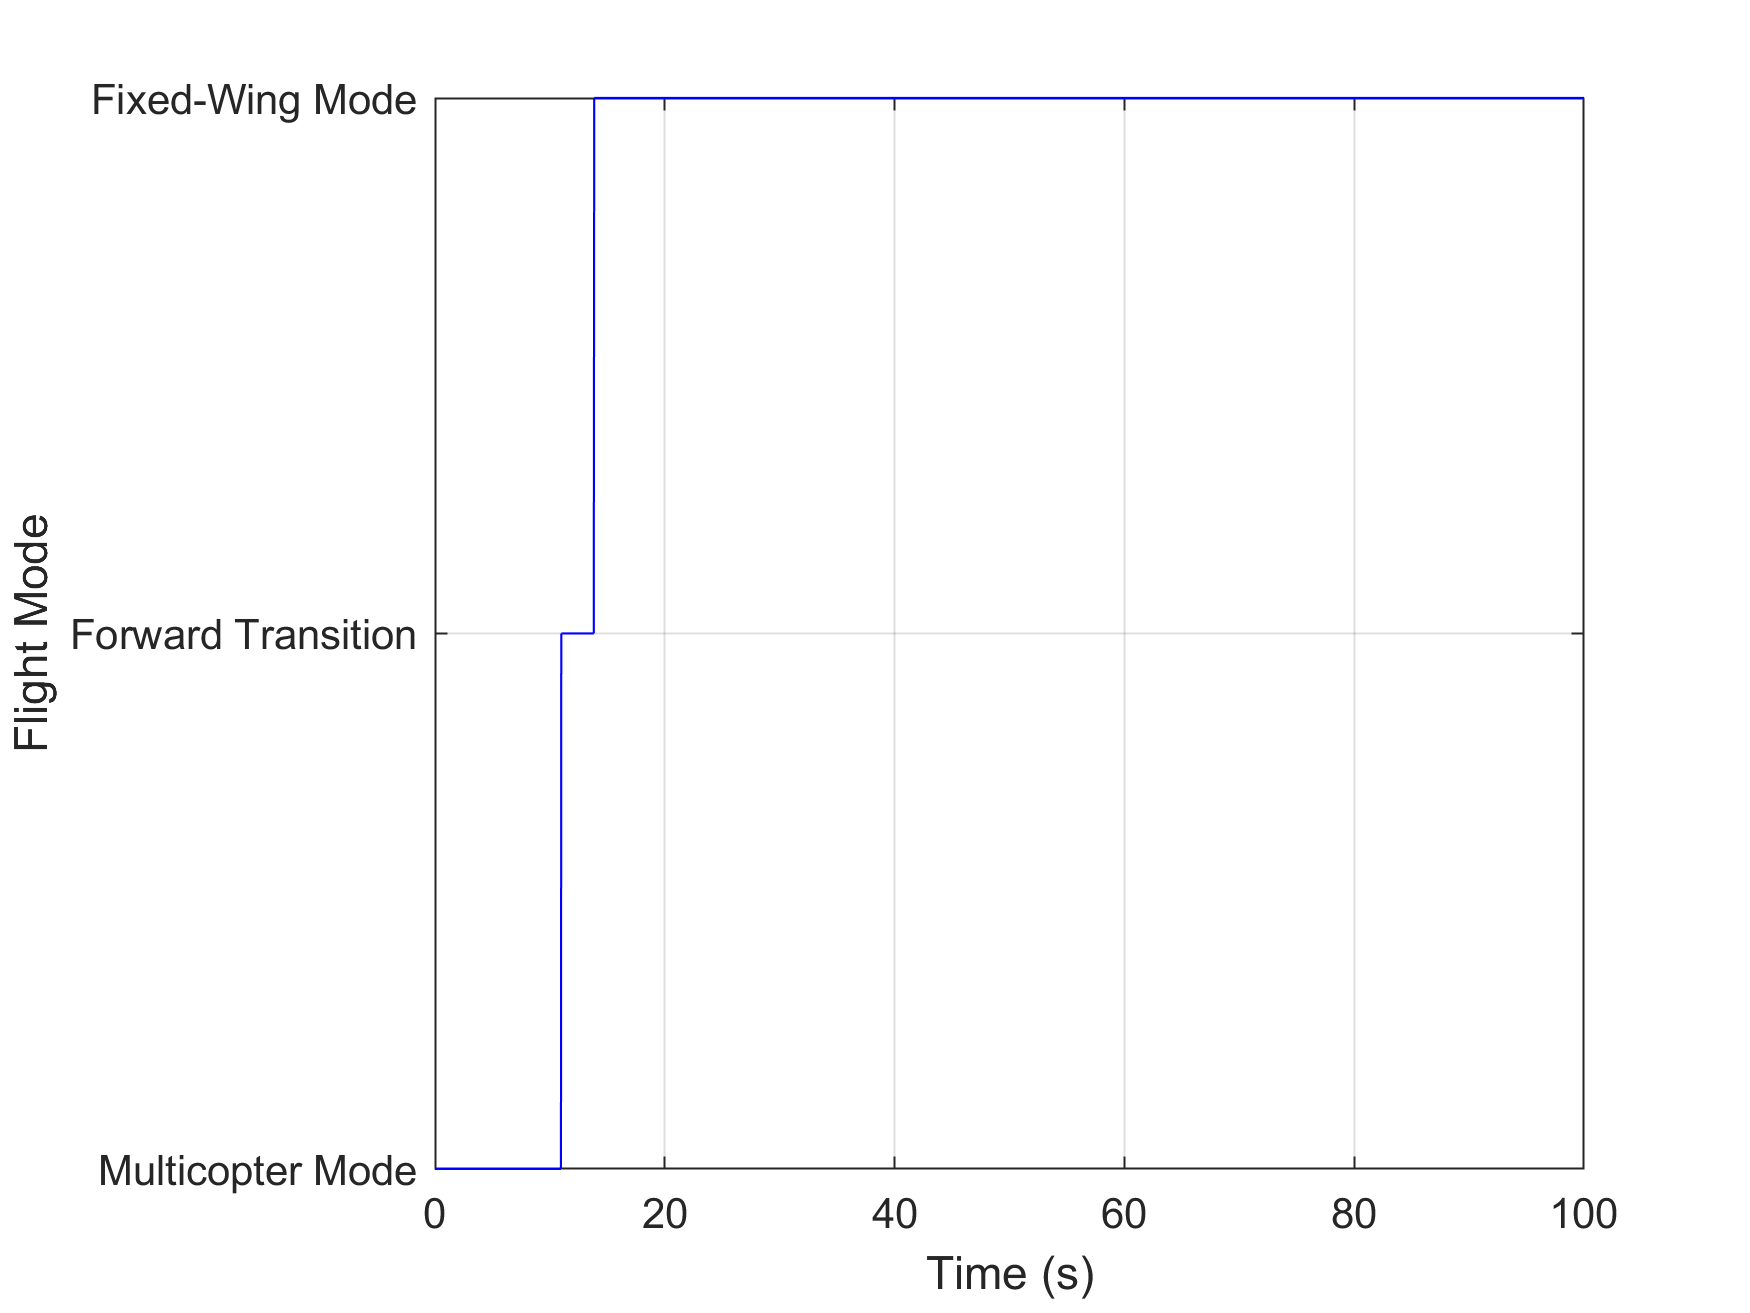
\includegraphics[width=0.8\textwidth]{flight_state_plot.png}
    \caption{Flight Mode Transition: Multicopter to Fixed-Wing Mode.}
    \label{fig:flight_state}
\end{figure}

In figure \ref{fig:flight_state}, 13.8 seconds is the time when the aircraft enters the fixed-wing mode. The transition phase is critical for the aircraft's stability and performance, and the neural network-based TECS gain tuning method significantly improves the aircraft's response during this phase.

\subsection{Energy Rate Error Response}
The energy rate error response is shown in Figure \ref{fig:ste_rate_error},\ref{fig:sbe_rate_error} . The neural network-based TECS demonstrates faster error reduction, leading to improved altitude and airspeed recovery and stability.
\begin{figure}[H]
    \centering
    \begin{minipage}{0.45\textwidth}
        \centering
        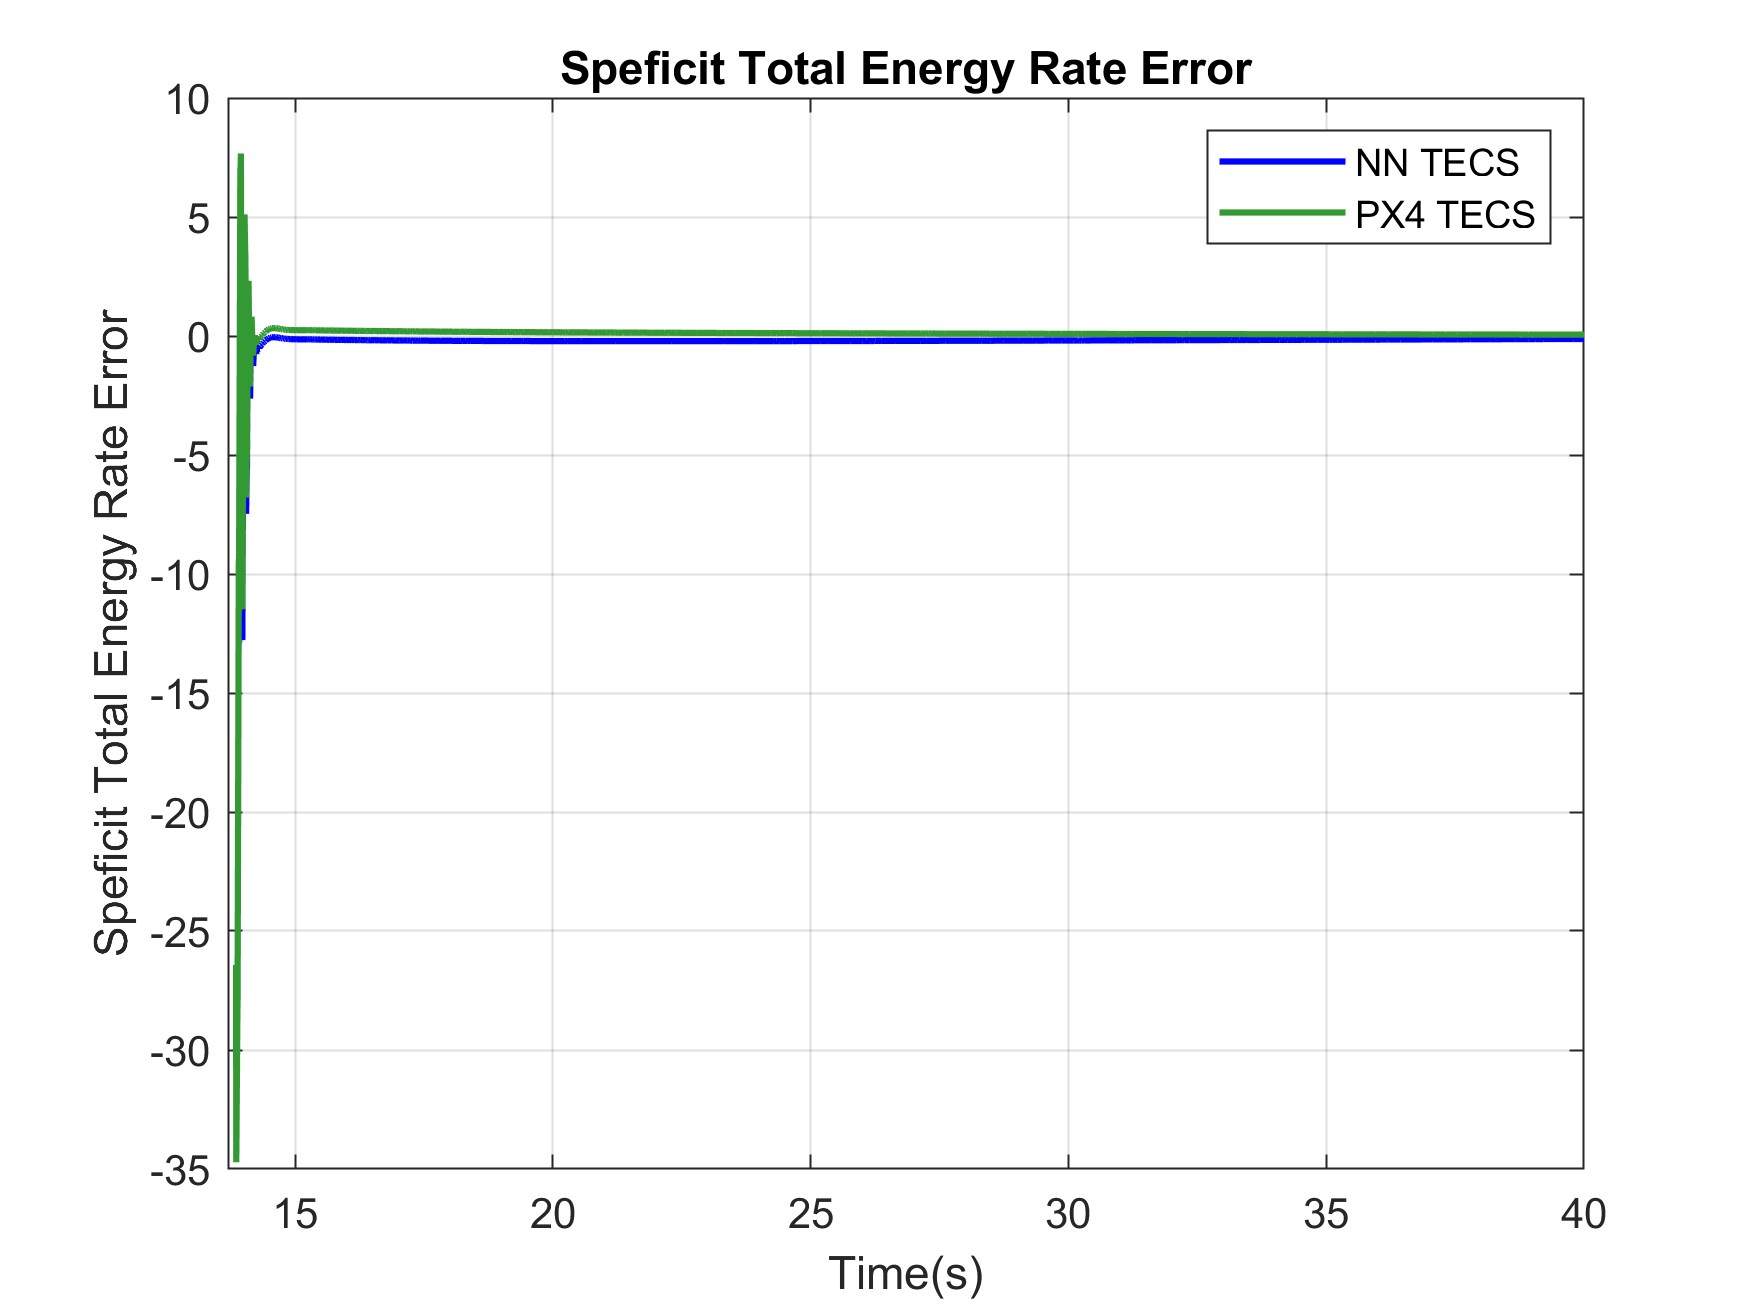
\includegraphics[width=\linewidth]{ste_rate_error_plot.png}
        \captionof{figure}{Specific Total Energy Rate Error (STE)}
        \label{fig:ste_rate_error}
    \end{minipage}
    \hfill
    \begin{minipage}{0.45\textwidth}
        \centering
        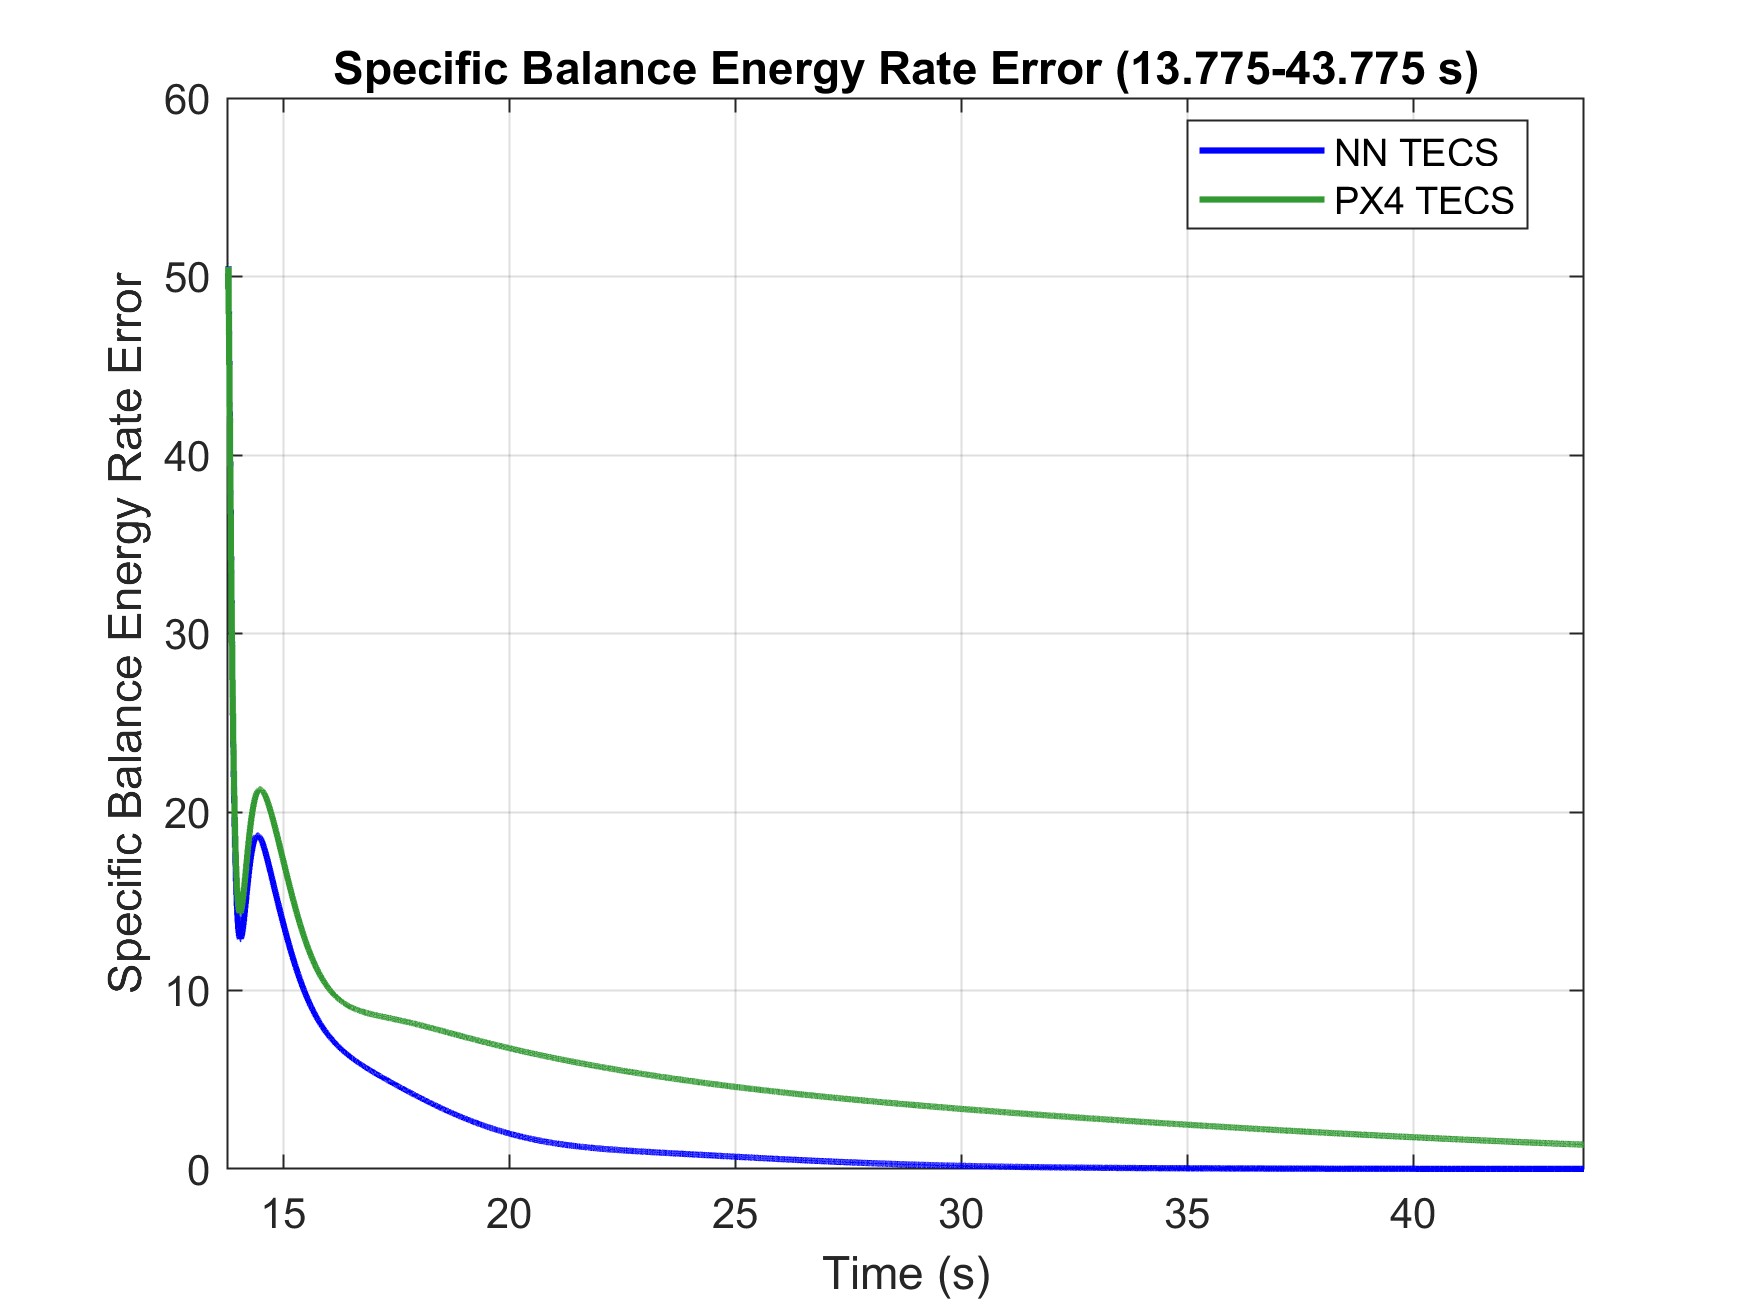
\includegraphics[width=\linewidth]{sbe_rate_error_plot.png}
        \captionof{figure}{Specific Balance Energy Rate Error (SBE)}
        \label{fig:sbe_rate_error}
    \end{minipage}
\end{figure}

\subsection{TECS Control Outputs}
Figure \ref{fig:thrust_output} and Figure \ref{fig:pitch_output} present the thrust and pitch outputs of the TECS control system, respectively. These plots illustrate the control inputs applied post-transition, highlighting the neural network's ability to adjust these outputs for improved stability.

\begin{figure}[H]
    \centering
    \begin{minipage}{0.45\textwidth}
        \centering
        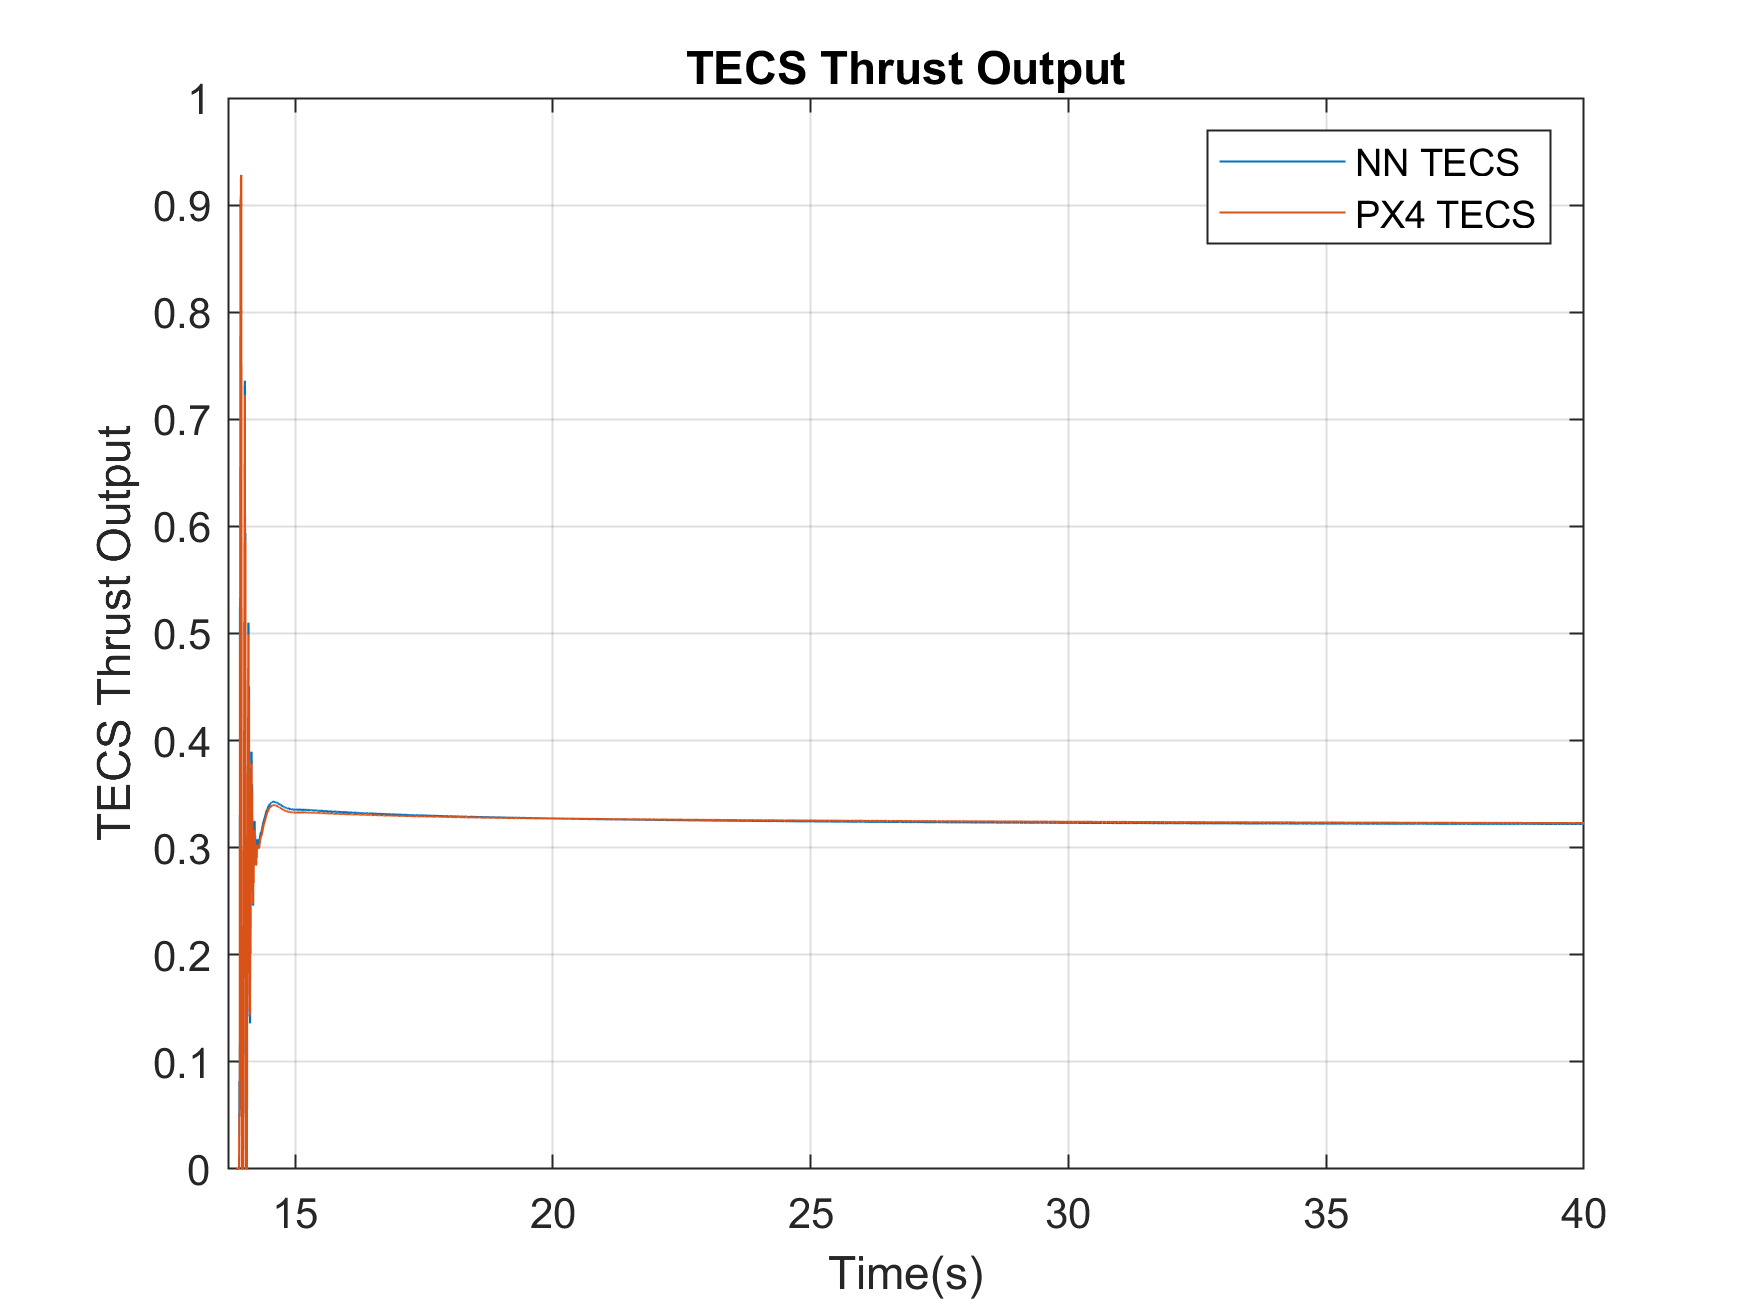
\includegraphics[width=\linewidth]{thrust_output_plot.png}
        \captionof{figure}{Thrust Output}
        \label{fig:thrust_output}
    \end{minipage}
    \hfill
    \begin{minipage}{0.45\textwidth}
        \centering
        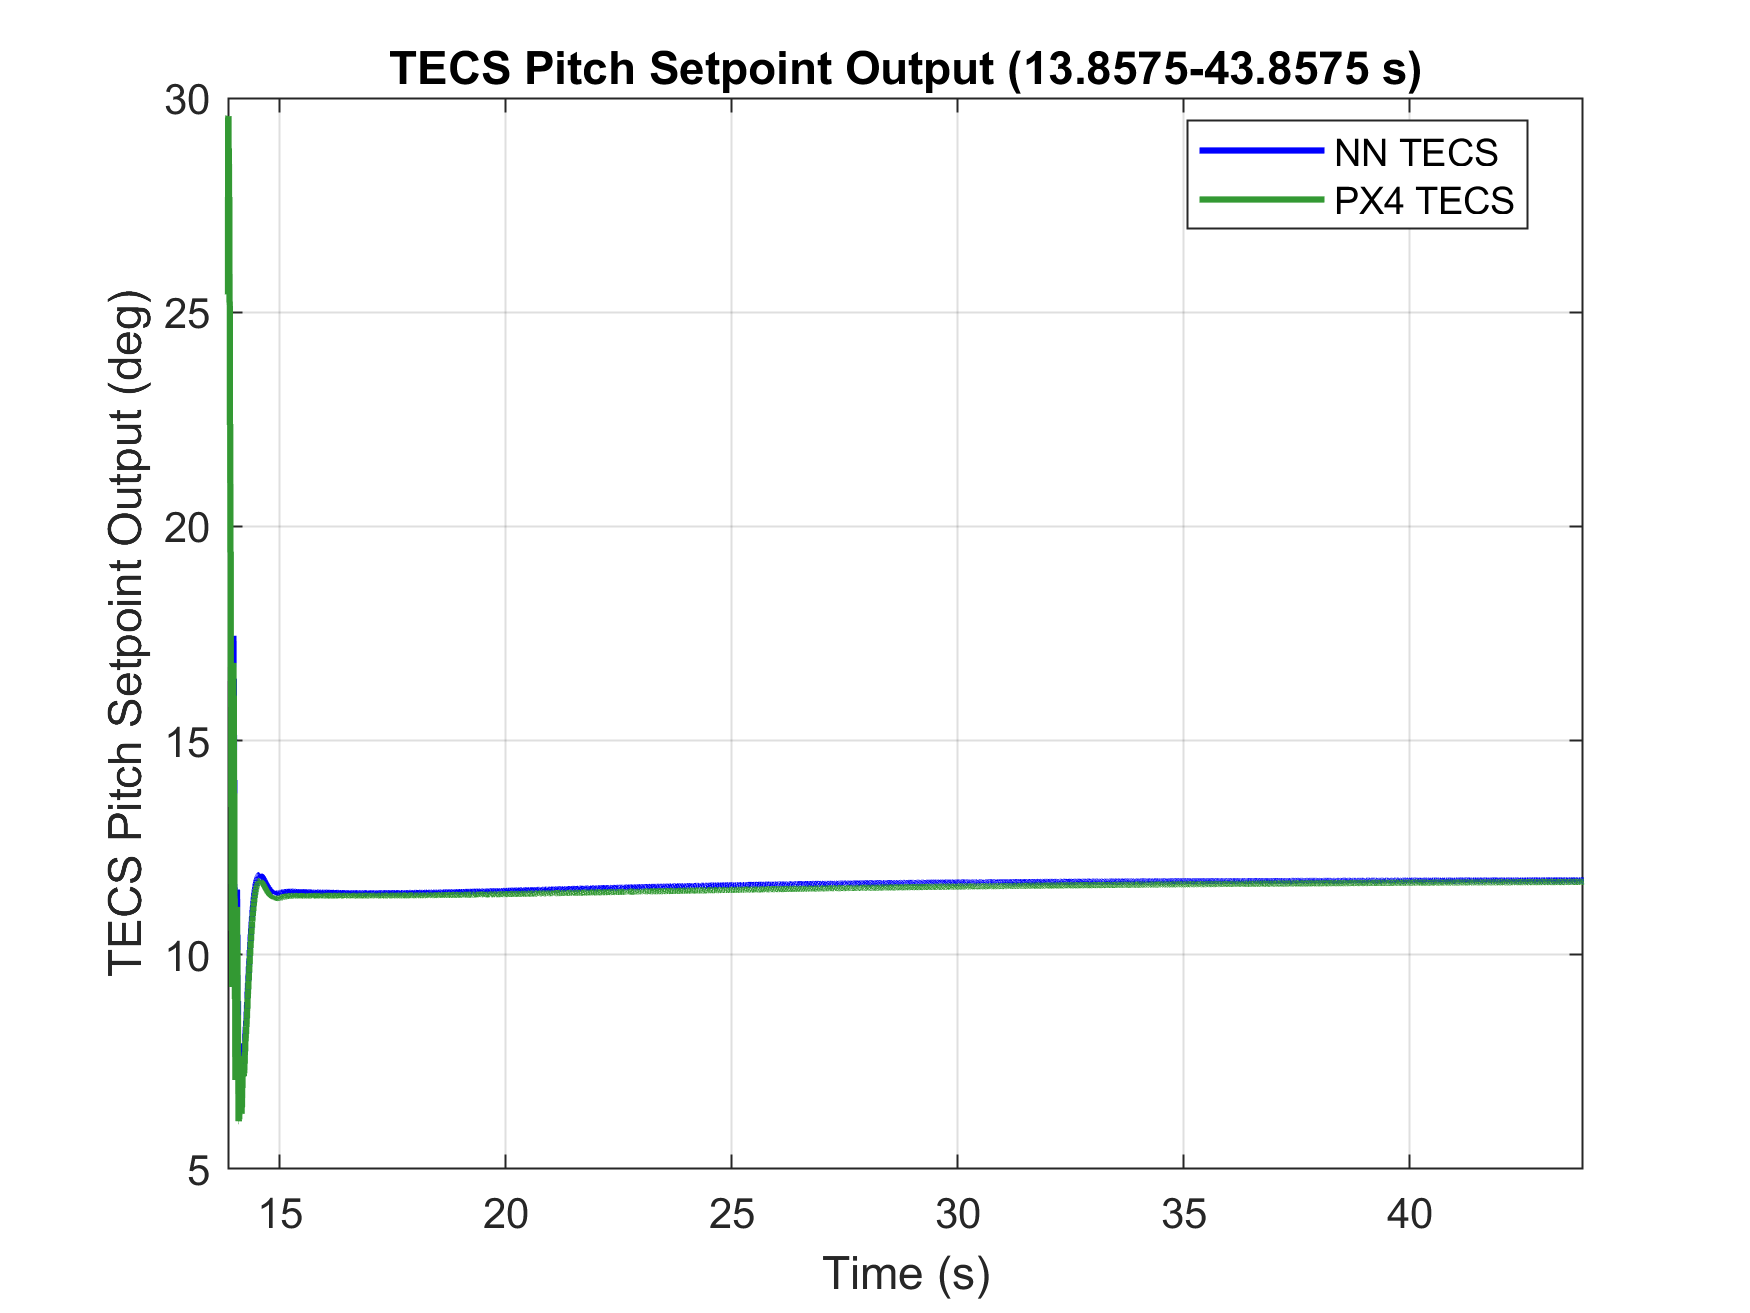
\includegraphics[width=\linewidth]{pitch_output_plot.png}
        \captionof{figure}{Pitch Output}
        \label{fig:pitch_output}
    \end{minipage}
\end{figure}


\subsection{Sensitive Analysis}
The neural network-based adaptive TECS gain tuning method was tested under various conditions to evaluate its robustness and sensitivity to different flight states. The results demonstrate consistent performance across different scenarios, highlighting the method's adaptability and reliability.

\begin{figure}[H]
    \centering
    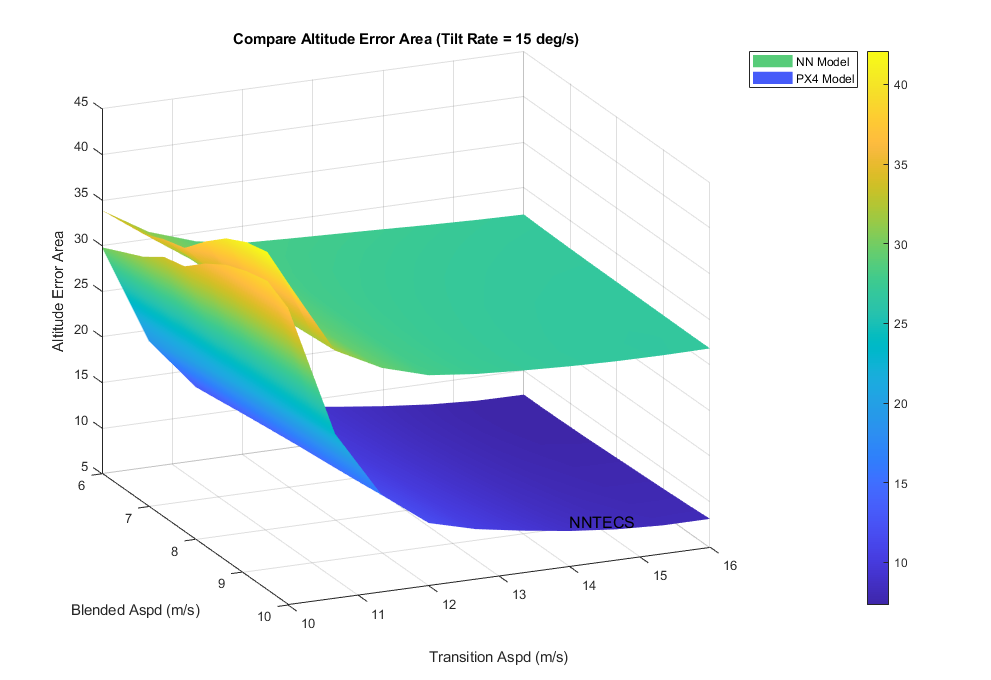
\includegraphics[width=0.8\textwidth]{sensitive_analysis.png}
    \caption{Sensitive Analysis: Neural Network TECS Performance under Different Flight States.}
    \label{fig:sensitive_analysis}
\end{figure}

%%%%%%%%%%%%%%%%%%%%%%%%%%%%%%%%%%%%%%%%%%
\section{Discussion}



%%%%%%%%%%%%%%%%%%%%%%%%%%%%%%%%%%%%%%%%%%
\section{Conclusions}

This section is not mandatory, but can be added to the manuscript if the discussion is unusually long or complex.

%%%%%%%%%%%%%%%%%%%%%%%%%%%%%%%%%%%%%%%%%%
\section{Patents}

%%%%%%%%%%%%%%%%%%%%%%%%%%%%%%%%%%%%%%%%%%
\vspace{6pt} 

%%%%%%%%%%%%%%%%%%%%%%%%%%%%%%%%%%%%%%%%%%
%% optional
%\supplementary{The following supporting information can be downloaded at:  \linksupplementary{s1}, Figure S1: title; Table S1: title; Video S1: title.}

% Only for journal Methods and Protocols:
% If you wish to submit a video article, please do so with any other supplementary material.
% \supplementary{The following supporting information can be downloaded at: \linksupplementary{s1}, Figure S1: title; Table S1: title; Video S1: title. A supporting video article is available at doi: link.}

% Only used for preprtints:
% \supplementary{The following supporting information can be downloaded at the website of this paper posted on \href{https://www.preprints.org/}{Preprints.org}.}

% Only for journal Hardware:
% If you wish to submit a video article, please do so with any other supplementary material.
% \supplementary{The following supporting information can be downloaded at: \linksupplementary{s1}, Figure S1: title; Table S1: title; Video S1: title.\vspace{6pt}\\
%\begin{tabularx}{\textwidth}{lll}
%\toprule
%\textbf{Name} & \textbf{Type} & \textbf{Description} \\
%\midrule
%S1 & Python script (.py) & Script of python source code used in XX \\
%S2 & Text (.txt) & Script of modelling code used to make Figure X \\
%S3 & Text (.txt) & Raw data from experiment X \\
%S4 & Video (.mp4) & Video demonstrating the hardware in use \\
%... & ... & ... \\
%\bottomrule
%\end{tabularx}
%}

%%%%%%%%%%%%%%%%%%%%%%%%%%%%%%%%%%%%%%%%%%
\authorcontributions{For research articles with several authors, a short paragraph specifying their individual contributions must be provided. The following statements should be used ``Conceptualization, X.X. and Y.Y.; methodology, X.X.; software, X.X.; validation, X.X., Y.Y. and Z.Z.; formal analysis, X.X.; investigation, X.X.; resources, X.X.; data curation, X.X.; writing---original draft preparation, X.X.; writing---review and editing, X.X.; visualization, X.X.; supervision, X.X.; project administration, X.X.; funding acquisition, Y.Y. All authors have read and agreed to the published version of the manuscript.'', please turn to the  \href{http://img.mdpi.org/data/contributor-role-instruction.pdf}{CRediT taxonomy} for the term explanation. Authorship must be limited to those who have contributed substantially to the work~reported.}

\funding{Please add: ``This research received no external funding'' or ``This research was funded by NAME OF FUNDER grant number XXX.'' and  and ``The APC was funded by XXX''. Check carefully that the details given are accurate and use the standard spelling of funding agency names at \url{https://search.crossref.org/funding}, any errors may affect your future funding.}

\institutionalreview{In this section, you should add the Institutional Review Board Statement and approval number, if relevant to your study. You might choose to exclude this statement if the study did not require ethical approval. Please note that the Editorial Office might ask you for further information. Please add “The study was conducted in accordance with the Declaration of Helsinki, and approved by the Institutional Review Board (or Ethics Committee) of NAME OF INSTITUTE (protocol code XXX and date of approval).” for studies involving humans. OR “The animal study protocol was approved by the Institutional Review Board (or Ethics Committee) of NAME OF INSTITUTE (protocol code XXX and date of approval).” for studies involving animals. OR “Ethical review and approval were waived for this study due to REASON (please provide a detailed justification).” OR “Not applicable” for studies not involving humans or animals.}

\informedconsent{Any research article describing a study involving humans should contain this statement. Please add ``Informed consent was obtained from all subjects involved in the study.'' OR ``Patient consent was waived due to REASON (please provide a detailed justification).'' OR ``Not applicable'' for studies not involving humans. You might also choose to exclude this statement if the study did not involve humans.

Written informed consent for publication must be obtained from participating patients who can be identified (including by the patients themselves). Please state ``Written informed consent has been obtained from the patient(s) to publish this paper'' if applicable.}

\dataavailability{We encourage all authors of articles published in MDPI journals to share their research data. In this section, please provide details regarding where data supporting reported results can be found, including links to publicly archived datasets analyzed or generated during the study. Where no new data were created, or where data is unavailable due to privacy or ethical restrictions, a statement is still required. Suggested Data Availability Statements are available in section ``MDPI Research Data Policies'' at \url{https://www.mdpi.com/ethics}.} 

% Only for journal Drones
%\durcstatement{Current research is limited to the [please insert a specific academic field, e.g., XXX], which is beneficial [share benefits and/or primary use] and does not pose a threat to public health or national security. Authors acknowledge the dual-use potential of the research involving xxx and confirm that all necessary precautions have been taken to prevent potential misuse. As an ethical responsibility, authors strictly adhere to relevant national and international laws about DURC. Authors advocate for responsible deployment, ethical considerations, regulatory compliance, and transparent reporting to mitigate misuse risks and foster beneficial outcomes.}

% Only for journal Nursing Reports
%\publicinvolvement{Please describe how the public (patients, consumers, carers) were involved in the research. Consider reporting against the GRIPP2 (Guidance for Reporting Involvement of Patients and the Public) checklist. If the public were not involved in any aspect of the research add: ``No public involvement in any aspect of this research''.}
%
%% Only for journal Nursing Reports
%\guidelinesstandards{Please add a statement indicating which reporting guideline was used when drafting the report. For example, ``This manuscript was drafted against the XXX (the full name of reporting guidelines and citation) for XXX (type of research) research''. A complete list of reporting guidelines can be accessed via the equator network: \url{https://www.equator-network.org/}.}
%
%% Only for journal Nursing Reports
%\useofartificialintelligence{Please describe in detail any and all uses of artificial intelligence (AI) or AI-assisted tools used in the preparation of the manuscript. This may include, but is not limited to, language translation, language editing and grammar, or generating text. Alternatively, please state that “AI or AI-assisted tools were not used in drafting any aspect of this manuscript”.}

\acknowledgments{This work was supported by Future Space Navigation \& Satellite Research Center through the National Research Foundation funded by the Ministry of Science and ICT, the Republic of Korea (2022M1A3C2074404). \\
This research was supported by Basic Science Research Program through the National Research Foundation of Korea(NRF) funded by the Ministry of Education(2020R1A6A1A03038540) \\
This work was supported by the IITP(Institute of Information \& Coummunications Technology Planning \& Evaluation)-ITRC(Information Technology Research Center) grant funded by the Korea government(Ministry of Science and ICT)(IITP-2025-RS-2024-00437494). }


\conflictsofinterest{Declare conflicts of interest or state ``The authors declare no conflicts of interest.'' Authors must identify and declare any personal circumstances or interest that may be perceived as inappropriately influencing the representation or interpretation of reported research results. Any role of the funders in the design of the study; in the collection, analyses or interpretation of data; in the writing of the manuscript; or in the decision to publish the results must be declared in this section. If there is no role, please state ``The funders had no role in the design of the study; in the collection, analyses, or interpretation of data; in the writing of the manuscript; or in the decision to publish the results''.} 

%%%%%%%%%%%%%%%%%%%%%%%%%%%%%%%%%%%%%%%%%%
%% Optional

%% Only for journal Encyclopedia
%\entrylink{The Link to this entry published on the encyclopedia platform.}

\abbreviations{Abbreviations}{
The following abbreviations are used in this manuscript:
\\

\noindent 
\begin{tabular}{@{}ll}
MDPI & Multidisciplinary Digital Publishing Institute\\
DOAJ & Directory of open access journals\\
TLA & Three letter acronym\\
LD & Linear dichroism
\end{tabular}
}

%%%%%%%%%%%%%%%%%%%%%%%%%%%%%%%%%%%%%%%%%%
%% Optional
\appendixtitles{no} % Leave argument "no" if all appendix headings stay EMPTY (then no dot is printed after "Appendix A"). If the appendix sections contain a heading then change the argument to "yes".
\appendixstart
\appendix
\section[\appendixname~\thesection]{}
\subsection[\appendixname~\thesubsection]{}
The appendix is an optional section that can contain details and data supplemental to the main text---for example, explanations of experimental details that would disrupt the flow of the main text but nonetheless remain crucial to understanding and reproducing the research shown; figures of replicates for experiments of which representative data are shown in the main text can be added here if brief, or as Supplementary Data. Mathematical proofs of results not central to the paper can be added as an appendix.

\begin{table}[H] 
\caption{This is a table caption.\label{tab5}}
%\newcolumntype{C}{>{\centering\arraybackslash}X}
\begin{tabularx}{\textwidth}{CCC}
\toprule
\textbf{Title 1}	& \textbf{Title 2}	& \textbf{Title 3}\\
\midrule
Entry 1		& Data			& Data\\
Entry 2		& Data			& Data\\
\bottomrule
\end{tabularx}
\end{table}

\section[\appendixname~\thesection]{}
All appendix sections must be cited in the main text. In the appendices, Figures, Tables, etc. should be labeled, starting with ``A''---e.g., Figure A1, Figure A2, etc.

%%%%%%%%%%%%%%%%%%%%%%%%%%%%%%%%%%%%%%%%%%
%\isPreprints{} % If the paper is ``preprints'', please uncomment this parenthesis.
%\printendnotes[custom] % Un-comment to print a list of endnotes

\reftitle{References}

% Please provide either the correct journal abbreviation (e.g. according to the “List of Title Word Abbreviations” http://www.issn.org/services/online-services/access-to-the-ltwa/) or the full name of the journal.
% Citations and References in Supplementary files are permitted provided that they also appear in the reference list here. 

%=====================================
% References, variant A: external bibliography
%=====================================
% \bibliography{your_external_BibTeX_file}

%=====================================
% References, variant B: internal bibliography
%=====================================

% ACS format
\isAPAandChicago{}{%
\begin{thebibliography}{999}
% Reference 1
\bibitem[Author1(year)]{ref-journal}
Author~1, T. The title of the cited article. {\em Journal Abbreviation} {\bf 2008}, {\em 10}, 142--149.
% Reference 2
\bibitem[Author2(year)]{ref-book1}
Author~2, L. The title of the cited contribution. In {\em The Book Title}; Editor 1, F., Editor 2, A., Eds.; Publishing House: City, Country, 2007; pp. 32--58.
% Reference 3
\bibitem[Author1 and Author2 (year)]{ref-book2}
Author 1, A.; Author 2, B. \textit{Book Title}, 3rd ed.; Publisher: Publisher Location, Country, 2008; pp. 154--196.
% Reference 4
\bibitem[Author4(year)]{ref-unpublish}
Author 1, A.B.; Author 2, C. Title of Unpublished Work. \textit{Abbreviated Journal Name} year, \textit{phrase indicating stage of publication (submitted; accepted; in press)}.
% Reference 5
\bibitem[Author8(year)]{ref-url}
Title of Site. Available online: URL (accessed on Day Month Year).
% Reference 6
\bibitem[Author6(year)]{ref-proceeding}
Author 1, A.B.; Author 2, C.D.; Author 3, E.F. Title of presentation. In Proceedings of the Name of the Conference, Location of Conference, Country, Date of Conference (Day Month Year); Abstract Number (optional), Pagination (optional).
% Reference 7
\bibitem[Author7(year)]{ref-thesis}
Author 1, A.B. Title of Thesis. Level of Thesis, Degree-Granting University, Location of University, Date of Completion.
\end{thebibliography}
}

% Chicago format (Used for journal: arts, genealogy, histories, humanities, jintelligence, laws, literature, religions, risks, socsci)
\isChicagoStyle{%
\begin{thebibliography}{9}
    \bibitem{hagan1999neural} Hagan, M. T., \& Demuth, H. B. (1999). Neural Networks for Control.
    \bibitem{ahn2005nonlinear} Ahn, K. K., \& Thanh, T. D. C. (2005). Nonlinear PID Control to Improve the Control Performance of the Pneumatic Artificial Muscle Manipulator Using Neural Network. \textit{Journal of Mechanical Science and Technology}, 19(1), 106-115.
    \bibitem{dao2000performance} Dao, V. N. P., \& Vemuri, R. (2000). A Performance Comparison of Different Back Propagation Neural Networks Methods in Computer Network Intrusion Detection.
\end{thebibliography}
}{}

% APA format (Used for journal: admsci, behavsci, businesses, econometrics, economies, education, ejihpe, games, humans, ijfs, journalmedia, jrfm, languages, psycholint, publications, tourismhosp, youth)
\isAPAStyle{%
\begin{thebibliography}{999}
% Reference 1
\bibitem[\protect\citeauthoryear{Azikiwe \BBA\ Bello}{{2020a}}]{ref-journal}
Azikiwe, H., \& Bello, A. (2020a). Title of the cited article. \textit{Journal Title}, \textit{Volume}(Issue), 
Firstpage--Lastpage/Article Number.
% Reference 2
\bibitem[\protect\citeauthoryear{Azikiwe \BBA\ Bello}{{2020b}}]{ref-book1}
Azikiwe, H., \& Bello, A. (2020b). \textit{Book title}. Publisher Name.
% Reference 3
\bibitem[Davison(1623/2019)]{ref-book2}
Davison, T. E. (2019). Title of the book chapter. In A. A. Editor (Ed.), \textit{Title of the book: Subtitle} 
(pp. Firstpage--Lastpage). Publisher Name. (Original work published 1623) (Optional).
% Reference 4
\bibitem[Fistek et al.(2017)]{ref-proceeding}
Fistek, A., Jester, E., \& Sonnenberg, K. (2017, Month Day). Title of contribution [Type of contribution]. Conference Name, Conference City, Conference Country.
% Reference 5
\bibitem[Hutcheson(2012)]{ref-thesis}
Hutcheson, V. H. (2012). \textit{Title of the thesis} [XX Thesis, Name of Institution Awarding the Degree].
% Reference 6
\bibitem[Lippincott \& Poindexter(2019)]{ref-unpublish}
Lippincott, T., \& Poindexter, E. K. (2019). \textit{Title of the unpublished manuscript} [Unpublished manuscript/Manuscript in prepara-tion/Manuscript submitted for publication]. Department Name, Institution Name.
% Reference 7
\bibitem[Harwood(2008)]{ref-url}
Harwood, J. (2008). \textit{Title of the cited article}. Available online: URL (accessed on Day Month Year).
\end{thebibliography}
}{}

% If authors have biography, please use the format below
%\section*{Short Biography of Authors}
%\bio
%{\raisebox{-0.35cm}{\includegraphics[width=3.5cm,height=5.3cm,clip,keepaspectratio]{Definitions/author1.pdf}}}
%{\textbf{Firstname Lastname} Biography of first author}
%
%\bio
%{\raisebox{-0.35cm}{\includegraphics[width=3.5cm,height=5.3cm,clip,keepaspectratio]{Definitions/author2.jpg}}}
%{\textbf{Firstname Lastname} Biography of second author}

% For the MDPI journals use author-date citation, please follow the formatting guidelines on http://www.mdpi.com/authors/references
% To cite two works by the same author: \citeauthor{ref-journal-1a} (\citeyear{ref-journal-1a}, \citeyear{ref-journal-1b}). This produces: Whittaker (1967, 1975)
% To cite two works by the same author with specific pages: \citeauthor{ref-journal-3a} (\citeyear{ref-journal-3a}, p. 328; \citeyear{ref-journal-3b}, p.475). This produces: Wong (1999, p. 328; 2000, p. 475)

%%%%%%%%%%%%%%%%%%%%%%%%%%%%%%%%%%%%%%%%%%
%% for journal Sci
%\reviewreports{\\
%Reviewer 1 comments and authors’ response\\
%Reviewer 2 comments and authors’ response\\
%Reviewer 3 comments and authors’ response
%}
%%%%%%%%%%%%%%%%%%%%%%%%%%%%%%%%%%%%%%%%%%
\PublishersNote{}
%\isPreprints{} % If the paper is ``preprints'', please uncomment this parenthesis.
\end{document}

